% Options for packages loaded elsewhere
\PassOptionsToPackage{unicode}{hyperref}
\PassOptionsToPackage{hyphens}{url}
\PassOptionsToPackage{dvipsnames,svgnames,x11names}{xcolor}
%
\documentclass[
  10pt,
]{scrartcl}
\title{Structured probabilistic coherence \linebreak and the usual counterexamples to probabilistic measures of coherence}
\author{}
\date{\vspace{-2.5em}}

\usepackage{amsmath,amssymb}
\usepackage{lmodern}
\usepackage{iftex}
\ifPDFTeX
  \usepackage[T1]{fontenc}
  \usepackage[utf8]{inputenc}
  \usepackage{textcomp} % provide euro and other symbols
\else % if luatex or xetex
  \usepackage{unicode-math}
  \defaultfontfeatures{Scale=MatchLowercase}
  \defaultfontfeatures[\rmfamily]{Ligatures=TeX,Scale=1}
\fi
% Use upquote if available, for straight quotes in verbatim environments
\IfFileExists{upquote.sty}{\usepackage{upquote}}{}
\IfFileExists{microtype.sty}{% use microtype if available
  \usepackage[]{microtype}
  \UseMicrotypeSet[protrusion]{basicmath} % disable protrusion for tt fonts
}{}
\makeatletter
\@ifundefined{KOMAClassName}{% if non-KOMA class
  \IfFileExists{parskip.sty}{%
    \usepackage{parskip}
  }{% else
    \setlength{\parindent}{0pt}
    \setlength{\parskip}{6pt plus 2pt minus 1pt}}
}{% if KOMA class
  \KOMAoptions{parskip=half}}
\makeatother
\usepackage{xcolor}
\IfFileExists{xurl.sty}{\usepackage{xurl}}{} % add URL line breaks if available
\IfFileExists{bookmark.sty}{\usepackage{bookmark}}{\usepackage{hyperref}}
\hypersetup{
  pdftitle={Structured probabilistic coherence and the usual counterexamples to probabilistic measures of coherence},
  colorlinks=true,
  linkcolor={blue},
  filecolor={blue},
  citecolor={blue},
  urlcolor={blue},
  pdfcreator={LaTeX via pandoc}}
\urlstyle{same} % disable monospaced font for URLs
\usepackage{longtable,booktabs,array}
\usepackage{calc} % for calculating minipage widths
% Correct order of tables after \paragraph or \subparagraph
\usepackage{etoolbox}
\makeatletter
\patchcmd\longtable{\par}{\if@noskipsec\mbox{}\fi\par}{}{}
\makeatother
% Allow footnotes in longtable head/foot
\IfFileExists{footnotehyper.sty}{\usepackage{footnotehyper}}{\usepackage{footnote}}
\makesavenoteenv{longtable}
\usepackage{graphicx}
\makeatletter
\def\maxwidth{\ifdim\Gin@nat@width>\linewidth\linewidth\else\Gin@nat@width\fi}
\def\maxheight{\ifdim\Gin@nat@height>\textheight\textheight\else\Gin@nat@height\fi}
\makeatother
% Scale images if necessary, so that they will not overflow the page
% margins by default, and it is still possible to overwrite the defaults
% using explicit options in \includegraphics[width, height, ...]{}
\setkeys{Gin}{width=\maxwidth,height=\maxheight,keepaspectratio}
% Set default figure placement to htbp
\makeatletter
\def\fps@figure{htbp}
\makeatother
\setlength{\emergencystretch}{3em} % prevent overfull lines
\providecommand{\tightlist}{%
  \setlength{\itemsep}{0pt}\setlength{\parskip}{0pt}}
\setcounter{secnumdepth}{5}
\newlength{\cslhangindent}
\setlength{\cslhangindent}{1.5em}
\newlength{\csllabelwidth}
\setlength{\csllabelwidth}{3em}
\newlength{\cslentryspacingunit} % times entry-spacing
\setlength{\cslentryspacingunit}{\parskip}
\newenvironment{CSLReferences}[2] % #1 hanging-ident, #2 entry spacing
 {% don't indent paragraphs
  \setlength{\parindent}{0pt}
  % turn on hanging indent if param 1 is 1
  \ifodd #1
  \let\oldpar\par
  \def\par{\hangindent=\cslhangindent\oldpar}
  \fi
  % set entry spacing
  \setlength{\parskip}{#2\cslentryspacingunit}
 }%
 {}
\usepackage{calc}
\newcommand{\CSLBlock}[1]{#1\hfill\break}
\newcommand{\CSLLeftMargin}[1]{\parbox[t]{\csllabelwidth}{#1}}
\newcommand{\CSLRightInline}[1]{\parbox[t]{\linewidth - \csllabelwidth}{#1}\break}
\newcommand{\CSLIndent}[1]{\hspace{\cslhangindent}#1}
%\documentclass{article}

% %packages
 \usepackage{booktabs}
\usepackage{subcaption}
\usepackage{multirow}
\usepackage{colortbl}
\usepackage{graphicx}
\usepackage{longtable}
\usepackage{ragged2e}

\usepackage{etex}
%\usepackage{yfonts}
\usepackage{marvosym}
\usepackage[notextcomp]{kpfonts}
\usepackage{nicefrac}
\newcommand*{\QED}{\hfill \footnotesize {\sc Q.e.d.}}
\usepackage{floatrow}
\usepackage[titletoc]{appendix}

\usepackage{tcolorbox}
%\renewcommand\thesubsection{\Alph{subsection}}

\usepackage[textsize=footnotesize]{todonotes}
\newcommand{\ali}[1]{\todo[color=gray!40]{#1}}
\newcommand{\mar}[1]{\todo[color=blue!40]{#1}}
\newcommand{\raf}[1]{\todo[color=olive!40]{#1}}
%\linespread{1.5}


\newcommand{\indep}{\!\perp \!\!\! \perp\!}
\newcommand{\s}[1]{\textsf{#1}}
\newcommand{\ms}[1]{\mathsf{#1}}



\setlength{\parindent}{10pt}
\setlength{\parskip}{1pt}


%language
%\usepackage{times}
\usepackage{mathptmx}
\usepackage[scaled=0.86]{helvet}
\usepackage{t1enc}
%\usepackage[utf8x]{inputenc}
%\usepackage[polish]{babel}
%\usepackage{polski}




%AMS
\usepackage{amsfonts}
\usepackage{amssymb}
\usepackage{amsthm}
\usepackage{amsmath}
\usepackage{mathtools}

\usepackage{geometry}
 \geometry{a4paper,left=35mm,top=20mm,}


%environments
\newtheorem{fact}{Fact}



%abbreviations
\newcommand{\ra}{\rangle}
\newcommand{\la}{\langle}
\newcommand{\n}{\neg}
\newcommand{\et}{\wedge}
\newcommand{\jt}{\rightarrow}
\newcommand{\ko}[1]{\forall  #1\,}
\newcommand{\ro}{\leftrightarrow}
\newcommand{\exi}[1]{\exists\, {_{#1}}}
\newcommand{\pr}[1]{\mathsf{P}(#1)}
\newcommand{\cost}{\mathsf{cost}}
\newcommand{\benefit}{\mathsf{benefit}}
\newcommand{\ut}{\mathsf{ut}}

\newcommand{\odds}{\mathsf{Odds}}
\newcommand{\ind}{\mathsf{Ind}}
\newcommand{\nf}[2]{\nicefrac{#1\,}{#2}}
\newcommand{\R}[1]{\texttt{#1}}
\newcommand{\prr}[1]{\mbox{$\mathtt{P}_{prior}(#1)$}}
\newcommand{\prp}[1]{\mbox{$\mathtt{P}_{posterior}(#1)$}}



\newtheorem{q}{\color{blue}Question}
\newtheorem{lemma}{Lemma}
\newtheorem{theorem}{Theorem}



%technical intermezzo
%---------------------

\newcommand{\intermezzoa}{
	\begin{minipage}[c]{13cm}
	\begin{center}\rule{10cm}{0.4pt}



	\tiny{\sc Optional Content Starts}
	
	\vspace{-1mm}
	
	\rule{10cm}{0.4pt}\end{center}
	\end{minipage}\nopagebreak 
	}


\newcommand{\intermezzob}{\nopagebreak 
	\begin{minipage}[c]{13cm}
	\begin{center}\rule{10cm}{0.4pt}

	\tiny{\sc Optional Content Ends}
	
	\vspace{-1mm}
	
	\rule{10cm}{0.4pt}\end{center}
	\end{minipage}
	}
%--------------------






















\newtheorem*{reply*}{Reply}
\usepackage{enumitem}
\newcommand{\question}[1]{\begin{enumerate}[resume,leftmargin=0cm,labelsep=0cm,align=left]
\item #1
\end{enumerate}}

\usepackage{float}

% \setbeamertemplate{blocks}[rounded][shadow=true]
% \setbeamertemplate{itemize items}[ball]
% \AtBeginPart{}
% \AtBeginSection{}
% \AtBeginSubsection{}
% \AtBeginSubsubsection{}
% \setlength{\emergencystretch}{0em}
% \setlength{\parskip}{0pt}






\usepackage[authoryear]{natbib}

%\bibliographystyle{apalike}



\usepackage{tikz}
\usetikzlibrary{positioning,shapes,arrows}

\usepackage{booktabs}
\usepackage{longtable}
\usepackage{array}
\usepackage{multirow}
\usepackage{wrapfig}
\usepackage{float}
\usepackage{colortbl}
\usepackage{pdflscape}
\usepackage{tabu}
\usepackage{threeparttable}
\usepackage{threeparttablex}
\usepackage[normalem]{ulem}
\usepackage{makecell}
\usepackage{xcolor}
\ifLuaTeX
  \usepackage{selnolig}  % disable illegal ligatures
\fi

\begin{document}
\maketitle

{
\hypersetup{linkcolor=blue}
\setcounter{tocdepth}{3}
\tableofcontents
}
\setlength{\abovedisplayskip}{-10pt}
\setlength{\belowdisplayskip}{5pt}

\pagebreak

\hypertarget{introduction-motivations}{%
\section{Introduction \& motivations}\label{introduction-motivations}}

The notion of coherence is often used in many philosophical, especially epistemological, discussions (for instance, in discussions about the truth-conduciveness of coherence). When we talk about the coherence of a set of propositions or about the coherence of a story, we seem to refer to how well their individual pieces fit together. How are we to understand and apply this notion systematically, though? In particular, we will be interested in probabilistic explications of this notion, as Bayesian epistemology strives to be a general epistemological project and as such it should be able to accommodate coherence-oriented considerations.

There is also a more practical reason to develop a better understanding of the notion: a plausible measure of coherence could be used to better evaluate the quality of some stories or narrations. For example in the legal context we would like to be able to assess the quality of a testimony in the court of law.\\
\todo{REFS}

Multiple probabilistic explications of coherence have been proposed
(Douven \& Meijs, 2007; Fitelson, 2003; Glass, 2002; Meijs \& Douven, 2007; Olsson, 2001; Roche, 2013; Shogenji, 1999). However, clear general principles to choose between them are hard to come by. One paper where some such principles have been formulated is (Schippers, 2014), where a list of seemingly plausible adequacy conditions for a coherence measure is proposed and shown to be inconsistent to argue for pluralism about the notion of coherence. However, some of those requirements are quite non-trivial.\footnote{Let us illustrate this. The (Dependence) condition formulated there requires that the coherence score of a set of propositions is above (below) the neutral score if for all pairs of non-empty subsets the posterior of an element of a pair conditional on the other element is higher than the prior of the former. This makes some of the features of the coherence measure dependent on the priors, and whether it should be so is not obvious. On the other hand, (Agreement) is formulated in terms of conditional probabilities between such pairs. If on a given measure \(\mathsf{P}\) all conditional probabilities (between pairs already mentioned) are higher than on \(\mathsf{P}'\), the coherence of a set given \(\mathsf{P}\) should be higher than given \(\mathsf{P}'\). The (Equivalence) requirement is that any finite set of logically equivalent propositions should be maximally coherent. This is suspicious, as the set \(\{ 0= 1, 2, = 5\}\) is a set of equivalent propositions (with sufficiently strong notion of logical equivalence in the background), but we would intuitively hesitate to say it's maximally coherent.}

The general point here is not that the approach taken in (Schippers, 2014) is flawed, but rather that the task of formulating general principles for coherence is a challenge, and that no clear list of such uncontroversial desiderata is on the horizon.

One approach to obtaining some clarity on which abstract conditions are plausible is looking at various thought experiments in which our intuitions about what the coherence scores should be (at least comparatively) are more robust than direct assessment of general requirements. In fact, looking at examples is what the main stream of literature on probabilistic coherence focused on, and each probabilistic measure of coherence faces a selection of seemingly intuitive counterexamples.

We decided to work with this methodology. We first gathered key examples that occur in the literature, represented them in terms of Bayesian networks, and developed \textbf{\textsf{R}} scripts calculating all coherence scores for the Bayesian networks at play, pushing further the results obtained by Koscholke (2016).\footnote{
  The whole work has been made possible by all those who contributed to the development of \textsf{\textbf{R}} language, and Marco Scutari, the author of \textsf{\textbf{bnlearn}} package, who was kind enough to extend his package with additional features upon our requests (Scutari \& Denis, 2015).} Then we reflected on the results, noticing that one weakness of the measures is that they pay little attention to the underlying structure of a given narration in the calculation of its coherence.

Inspired by this observation, we formulate our own proposal, which diverges from the known purely probabilistic measures of coherence in three important respects: (i) It is not a function of a probability measure and a set
of propositions alone, because it is also sensitive to the selection and direction of edges in a Bayesian network representing an agent's credal state. (ii) Unlike in the case of quite a few coherence measures, it is sensitive to
the weakest links in the narration. (iii) It is not obtained by simply averaging confirmation levels between all possible combinations of elements.

We described this approach in a more detailed introduction to this measure {[}ANONYMIZED{]}, which explains the method and some of the theoretical decisions that we have made, and show how it works using a Bayesian network developed for the well-known Sally Clark case (Fenton \& Neil, 2018). The goal of the current paper is to discuss a range of philosophical counterexamples to the existing probabilistic measures of coherence and evaluate the performance of our approach using those as a benchmark, arguing that it performs much better than the existing ones.

Accordingly, in Section \ref{sec:measures} we introduce all the coherence measures, including the key motivations for and a pseudo-code description of our measure. In Section \ref{sec:examples} we describe the thought experiments meant as counterexamples to coherence measures, their corresponding desiderata and their status on various coherence measures, including ours. The order of the discussion of any given example is straightforward: we first explain what the situation we are to consider is, what the intuitive desiderata related to it are supposed to be, how the situation is represented by means of a Bayesian network(s), and what happens when we apply all coherence measures. We end with Section \ref{sec:discussion} in which we compare all of the results and draw some general conclusions.

\hypertarget{probabilistic-coherence-measures-and-structured-coherence}{%
\section{Probabilistic coherence measures and structured coherence}\label{probabilistic-coherence-measures-and-structured-coherence}}

\label{sec:measures}

Quite a few different measures of coherence have been proposed in the literature. Two early proposals are:

\begin{itemize}
\tightlist
\item
  Shogenji's
  \textbf{deviation from independence} (Shogenji, 1999), is defined as the ratio between the probability of the
  conjunction of all claims, and the probability that the conjunction
  would get if all its conjuncts were probabilistically independent (scaling from 0 to \(\infty\) with neutral point 1):
\end{itemize}

\begin{align}
    \tag{Shogenji}
    \label{coh:Shogenji}
     \mathcal{C}_{S}(S)=\frac{P(\bigwedge S)}{\prod_{i=1}^{\vert S \vert}\{P(S_i)\vert i \in S\}}
\end{align}

\noindent This measure was later generalized by Meijs \& Douven (2007). According to this approach, \eqref{coh:Shogenji} is applied not only to the whole set of propositions, but to each non-empty non-singleton subset of the set, and the final value is defined as the average of all sub-values thus obtained.

\begin{itemize}
\tightlist
\item
  \textbf{Relative overlap} (Glass, 2002; Olsson, 2001), is defined as the ratio between the intersection of all propositions and their union (scaling from -1 to 1 with no clear neutral point):
\end{itemize}

\begin{align}
    \tag{Olsson}
    \label{coh:Olsson}
    \mathcal{C}_{O}(S)=\frac{P(\bigwedge S)}{P(\bigvee S)}
\end{align}

\noindent It has also been generalized in a way analogous to the one used in the generalization of the Shogenji's measure (Meijs \& Douven, 2007).

Both of these approaches are susceptible to various objections and counterexamples (Akiba, 2000; Bovens \& Hartmann, 2004; Crupi, Tentori, \& Gonzalez, 2007; Koscholke, 2016; Merricks, 1995; Schippers \& Koscholke, 2019; Shogenji, 1999, 2001, 2006; Siebel, 2004, 2006). To overcome them, more recent works proposed \textbf{average mutual support} measures, starting with (Fitelson, 2003). The general recipe for such measures is as follows.

\begin{itemize}
\item
  Given that \(S\) is a set whose coherence is to be measured, let \(P\)
  indicate the set of all ordered pairs of non-empty, disjoint subsets
  of \(S\).
\item
  First, define a confirmation function (of  a hypothesis \(H\) by evidence  \(E\)): \(\mathsf{conf}(H,E)\).
\item
  For each pair \(\langle X, Y \rangle \in P\), calculate
  \(\mathsf{conf}(\bigwedge X, \bigwedge Y)\), where $\bigwedge X$  is the conjunction of all the elements of $X$ (and $\bigwedge Y$ is to be understood analogously).
\item
  Take the mean of all the results:
\end{itemize}

\begin{align*}
    \mathcal{C}(S) & =
\mathsf{mean}\left(\left\{\mathsf{conf}(\bigwedge X_i, \bigwedge Y_i) | \langle X_i, Y_i \rangle \in P\right\} \right).
\end{align*}

\noindent Different measures of coherence result from different choices of a confirmation measure. Here are the key candidates present in the literature:

\begin{itemize}
\tightlist
\item
  Fitelson (2003) uses the following confirmation function (the resulting coherence measure ranges from -1 to 1 with neutral point at 0):
\end{itemize}

\begin{align}
    F(H,E) & = \begin{cases}
    1 & E\models H, E\not \models \bot \\
    -1 & E \models \neg H\\
    \frac{P(E|H)-P(E|\neg H)}{P(E|H)+P(E|\neg H)} & \mbox{o/w}
    \end{cases} \nonumber \\
\tag{Fitelson}  
    \mathcal{C}_{F}(S) & =
\mathsf{mean}\left(\left\{F(\bigwedge X_i, \bigwedge Y_i) | \langle X_i, Y_i\rangle \in P\right\} \right)
\end{align}

\begin{itemize}
\tightlist
\item
  Douven \& Meijs (2007) use the difference confirmation measure (with coherence ranging from -1 to 1 with neutral point at 0):
\end{itemize}

\begin{align}
    D(H,E) &= P(H|E) - P(H) \nonumber \\
\tag{DM}  
    \mathcal{C}_{DM}(S) & =
\mathsf{mean}\left(\left\{D(\bigwedge X_i, \bigwedge Y_i) | \langle X_i, Y_i\rangle \in P\right\} \right)
\end{align}

\begin{itemize}
\tightlist
\item
  Roche (2013) uses the absolute confirmation measure
  (the resulting coherence measure ranges from 0 to 1 with neutral point at \(0.5\)):
\end{itemize}

\begin{align} \nonumber 
    A(H,E)  & = \begin{cases}
    1 & E\models H, E\not \models \bot \\
    0 & E \models \neg H\\
    P(H|E) & \mbox{o/w} \\
    \end{cases} \\
\tag{Roche}  
    \mathcal{C}_{R}(S) & =
\mathsf{mean}\left(\left\{A(\bigwedge X_i, \bigwedge Y_i) | \langle X_i, Y_i\rangle \in P\right\} \right) 
\end{align}

Mind your head: different measures use different scales and have different neutral points (values taken for any set of probabilistically independent propositions; not all measures have neutral points). This is worth keeping in mind when it comes to various desiderata that we will discuss.

As we already mentioned in the introduction, formulating abstract formal requirements for a coherence measure and investigating whether a given coherence measure satisfies them has not resulted in an agreement. For this reason, we follow another path, which has dominated the literature on the topic. We look at how the measures behave in test scenarios. Many putative scenarios were put forward as counterexamples. They usually have the form of a few propositions formulated in natural language, such that intuitive judgments of coherence involved and the formal coherence calculations seem to diverge (Akiba, 2000; Bovens \& Hartmann, 2004; Koscholke, 2016; Meijs \& Douven, 2007, 2007; Merricks, 1995; Schippers \& Koscholke, 2019, 2019; Shogenji, 1999, 2001, 2006; Siebel, 2004, 2006). We will focus on these examples in what follows. To spoil the experience, let us already point out that the probabilistic measures we introduced above do not seem to handle these examples very well (read on for details).

Inspired by these failures, in {[}REFERENCE SUPRESSED FOR ANONYMITY{]} we proposed to take a different perspective. Putting the earliest measures aside (they were problematic for various reasons), we noticed that the problems with the average mutual support measures stem from the fact that the coherence score is an average confirmation score for all possible combinations of the parts of a narration. Therefore we proposed to take a more fine-grained account. First, we represented an agent's belief state by means of a Bayesian network, which comprises not only a probabilistic measure but additional structural information, Then we used this structural information in our definition of coherence, so that only those directions of support are considered which in fact are indicated by the structure of the agent's belief state.

While we refer the reader to a more extensive treatment in {[}REFERENCE SUPRESSED FOR ANONYMITY{]}, we now briefly discuss the main idea behind it. A Bayesian network represents agent's probabilistic belief state with respect to the relevant nodes. Some of them are distinguished as fixed narration nodes---the agent holds definite beliefs about which states of these nodes occur.

Each parented node in the BN receives its expected confirmation score (\s{ECS}). It is calculated by looking at all combinations of its states and states of its parents not excluded by agents' fixed beliefs. For each of these combinations, the confirmation score between the parents' states and the child state is calculated (in the pseudo-code, we use confirmation measure \s{Z}, in further calculations we also use measures \s{LR} and \s{L} for comparison)\footnote{DEFINITIONS}. Then, a weighted average of these scores is obtained, where weights are the probabilities of the combinations of parents' states obtained by updating the BN with the fixed states of the fixed narration nodes. The final coherence score is either the mean of the \s{ecs} scores, if all of them are positive, or it is a weighted average of their mean and their minimum, \((1- |\s{min}(\s{ecs})|) \times \s{mean}(\s{ecs}) + |\s{min}(\s{ecs})| \times \s{min}(\s{ecs})\), otherwise.\footnote{We have developed \textbf{\textsf{R}} code calculating this and other measures to handle calculations that will be discussed further on, the code with documentation is available at ANONYMIZED.}

\pagebreak 
\footnotesize

\begin{verbatim}
FUNCTION parents_child_possible_states(parents,child)
    IF child included in narration THEN
        consequentStates <- the unique state of child as reported in the narration
    ELSE
        consequentStates <- all possible states of child
    FOR EACH parent in parents
        IF parent included in narration THEN
            parentStates[parent] <- the unique state of parent as reported in the narration
        ELSE
            parentStates[parent] <- all possible states of parent
    parentsStates <- all combinations of parentStates
    variants <- list of all possible combinations of consequentStates and parentsStates
    RETURN variants


FUNCTION coherence_from_ecs(ecs)
    IF min(ecs) <= 0 THEN
        RETURN mean(ecs) * (min(ecs)+1) - min(ecs)min(ecs)
        #this is equivalent to (1- |min(ecs)|) * mean(ecs) + |min(ecs)| * min(ecs)
    ELSE
        RETURN mean(ecs)

FUNCTION structured_coherence(BN,fixedNodes,fixedStates)
    parentedNodes <- vector of non-root nodes in BN
    ecsList <- []
    FOR EACH parentedNode IN parentedNodes
        variants <- parents_child_possible_states(parents,parentedNode)
        variants_count <- length(variants)
        sumParentsNarr <- 0
        FOR EACH variant IN variants
            childPrior <- prior probability of the child state in variant
            childPosterior <- posterior probability of the child state in variant,
                        obtained by updating on the parents states
                        from this variant
            parentsNarr[variant] <- joint probability of 
                        the parents states in variant in BN updated with fixedStates of fixedNodes
            sumParentsNarr <- sumParentsNarr +  parentsNarr[variant] 
            z[variant] <- z_confirmation_measure(childPrior, childPosterior)
        ecs <- 0  #expected confirmation score
        FOR EACH variant IN variants
            IF parentsNarr[variant] > 0 THEN
                weight <- parentsNarr[variant]/sumParentsNarr
            ELSE
                weight <- 1/variants_count
            zScaled <- z[variant] * weight
            ecs <- ecs + zScaled
        ecsList.add(ecs)
    RETURN coherence_from_ecs(ecsList)
\end{verbatim}

\normalsize

\noindent Having introduced the coherence measures at play, let us now move to the key counterexamples discussed in the literature.

\hypertarget{challenges-and-their-treatment}{%
\section{\texorpdfstring{Challenges and their treatment \label{sec:examples}}{Challenges and their treatment }}\label{challenges-and-their-treatment}}

For each of the counterexamples, we first explain what it is and what the connected desiderata are. Then we represent it as a Bayesian network, and finally we use our \textbf{\textsf{R}} scripts to calculate coherence scores that the coherence measures included in the previous section (including ours) yield for a given example and whether the desiderata are satisfied.
Here are the counterexamples put forward against various coherence measures in the literature. We ignored only a few where both we didn't share the authors' intuitions and the examples were not picked up in further discussion in the literature.

\hypertarget{penguins}{%
\subsection{Penguins}\label{penguins}}

\textbf{The scenario.} A challenge discussed in (Bovens \& Hartmann, 2004, p. 50) and (Meijs \& Douven, 2007) consists of the propositions (instead of \emph{letters} or \emph{abbreviations}, we'll talk about \emph{nodes}, as these will be used later on in Bayesian networks) displayed in Table \ref{tab:penguinsPropositions}.

\begin{table}[H]

\caption{\label{tab:penguinsPropositions}Propositions in the Penguins scenario}
\centering
\begin{tabular}[t]{ll}
\toprule
node & content\\
\midrule
\cellcolor{gray!6}{B} & \cellcolor{gray!6}{Tweety is a bird.}\\
G & Tweety is a grounded animal.\\
\cellcolor{gray!6}{P} & \cellcolor{gray!6}{Tweety is a penguin.}\\
\bottomrule
\end{tabular}
\end{table}

\noindent \textbf{Desiderata.}
It seems that the set \{\s{B},\s{G}\}, which doesn't contain the information about Tweety being a penguin, should be less coherent than the one that does contain this information: \{\s{B},\s{G},\s{P}\}.

\vspace{2mm}\begin{description}
    \item[(\s{BG}$<$\s{BGP})] \{\s{B},\s{G}\}  should be less coherent than \{\s{B},\s{G},\s{P}\}. 
\end{description}\vspace{2mm}

Another intuition about this scenario (Schippers \& Koscholke, 2019) is that when you consider a set which says that Tweety is both a bird and a penguin: \{\s{B},\s{P}\}, adding proposition about not flying (\s{G}) shouldn't increase the coherence of the set as much as moving from \{\s{B},\s{G}\} to \{\s{B},\s{G}, \s{P}\}. It's a well-known fact that penguins don't fly and by adding \s{G} explicitly to the set, one wouldn't gain as much information.
However, as \s{G} is not a logical consequence of \s{P}, it can be argued that \{\s{B},\s{P}\} and \{\s{B},\s{P},\s{G}\} represent different information sets, and so some difference in their coherence is to be expected.

\vspace{2mm}\begin{description}
    \item[(\s{BG} $\ll$ \s{BP}$\leq$\s{BGP})]  \{\s{B},\s{P}\} should be notably above  \{\s{B},\s{G}\}, and less than \{\s{B},\s{P},\s{G}\}.
\end{description}\vspace{2mm}

\noindent Formally, we'll require that the absolute difference between \s{BG} and \s{BP} be greater than \(.1\) (the exact placement of the threshold doesn't make a huge difference, unless it's at an unintuitive value below \(.01\)) and that \{\s{B},\s{G}\} \(\leq\) \{\s{B},\s{P},\s{G}\}.

\noindent \textbf{Bayesian network.} We used the distribution used in the original formulation to build a BN corresponding to the narrations at play (Fig. \ref{fig:BGP}).\footnote{Not without concerns. There are around 18 000 species of birds, and around 60 of them are flightless. We  couldn't find information about counts, but it seems the probability of being a penguin if one is grounded is overestimated by philosophers.  Also, there are many things that are not grounded but are not birds, mostly insects, and there's plenty of them. We did spend some time coming up with plausible ranges of probabilities to correct for such factors, and none of them actually makes a difference to the main point. So, for the sake of simplicity, we leave the original unrealistic distribution in our discussion.}

\begin{figure}[H]
\hspace{2cm}\scalebox{0.7}{\begin{subfigure}[!ht]{0.4\textwidth}

\begin{center}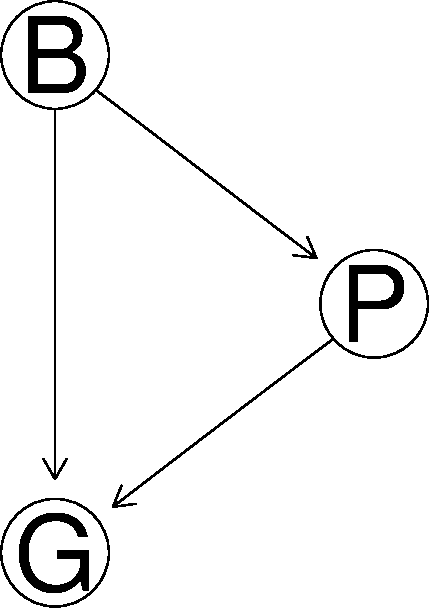
\includegraphics[width=1\linewidth]{coherencePaper32_files/figure-latex/unnamed-chunk-2-1} \end{center}
\end{subfigure}} \hfill
\hspace{-3cm}\scalebox{0.8}{\begin{subfigure}[!ht]{0.4\textwidth}

\begin{tabular}{lr}
\toprule
B & Pr\\
\midrule
1 & 0.5\\
0 & 0.5\\
\bottomrule
\end{tabular}


\begin{tabular}{lrr}
\toprule
\multicolumn{1}{c}{P} & \multicolumn{2}{c}{B} \\
  & 1 & 0\\
\midrule
1 & 0.02 & 0\\
0 & 0.98 & 1\\
\bottomrule
\end{tabular}


\begin{tabular}{lllr}
\toprule
\multicolumn{1}{c}{} & \multicolumn{1}{c}{B} & \multicolumn{1}{c}{P} & \multicolumn{1}{c}{} \\
G &  &  & Pr\\
\midrule
1 & 1 & 1 & 1.00\\
0 & 1 & 1 & 0.00\\
1 & 0 & 1 & 0.00\\
0 & 0 & 1 & 1.00\\
1 & 1 & 0 & 0.00\\
0 & 1 & 0 & 1.00\\
1 & 0 & 0 & 0.98\\
0 & 0 & 0 & 0.02\\
\bottomrule
\end{tabular}
\end{subfigure}}
\caption{Bayesian network for the Penuins problem.}
\label{fig:BGP}
\end{figure}

\noindent \textbf{Results.} Now, let's calculate the coherence scores (Table \ref{tab:penguinsCoherence}) and see if the desiderata are satisfied (Table \ref{tab:penguinsDesiderata}). The measures are: Olsson-Glass, generalized Olsson-Glass, Shogenji, generalized Shogenji, Douven-Meijs, Roche, Fitelson, Structured with Z, LR, and L used as a confirmation measure.

\begin{table}[H]

\caption{\label{tab:penguinsCoherence}Coherence scores for the Penguins scenario (rounded). Note how LR might result in Inf if a conditional probability of 1 at an arrow used in the calculations is involved.}
\centering
\resizebox{\linewidth}{!}{
\begin{tabular}[t]{lrrrrrrrrrr}
\toprule
  & OG & OGGen & Sh & ShG & DM & R & Fi & SZ & SLR & SL\\
\midrule
\cellcolor{gray!6}{Penguins: BGP 111} & \cellcolor{gray!6}{0.01} & \cellcolor{gray!6}{0.015} & \cellcolor{gray!6}{4.00} & \cellcolor{gray!6}{2.01} & \cellcolor{gray!6}{0.255} & \cellcolor{gray!6}{0.51} & \cellcolor{gray!6}{0.453} & \cellcolor{gray!6}{0.505} & \cellcolor{gray!6}{Inf} & \cellcolor{gray!6}{0.669}\\
Penguins: BG 11 & 0.01 & 0.010 & 0.04 & 0.04 & -0.480 & 0.02 & -0.960 & -0.960 & 0.02 & -0.960\\
\cellcolor{gray!6}{Penguins: BP 11} & \cellcolor{gray!6}{0.02} & \cellcolor{gray!6}{0.020} & \cellcolor{gray!6}{2.00} & \cellcolor{gray!6}{2.00} & \cellcolor{gray!6}{0.255} & \cellcolor{gray!6}{0.51} & \cellcolor{gray!6}{0.669} & \cellcolor{gray!6}{0.010} & \cellcolor{gray!6}{2.02} & \cellcolor{gray!6}{0.338}\\
\bottomrule
\end{tabular}}
\end{table}

\begin{table}[H]

\caption{\label{tab:penguinsDesiderata}Desiderata satisfaction for the Penguins scenario.}
\centering
\resizebox{\linewidth}{!}{
\begin{tabular}[t]{lllllllllll}
\toprule
  & OG & OGGen & Sh & ShG & DM & R & Fi & SZ & SLR & SL\\
\midrule
\cellcolor{gray!6}{Penguins: BG$<$BGP} & \cellcolor{gray!6}{FALSE} & \cellcolor{gray!6}{TRUE} & \cellcolor{gray!6}{TRUE} & \cellcolor{gray!6}{TRUE} & \cellcolor{gray!6}{TRUE} & \cellcolor{gray!6}{TRUE} & \cellcolor{gray!6}{TRUE} & \cellcolor{gray!6}{TRUE} & \cellcolor{gray!6}{FALSE} & \cellcolor{gray!6}{TRUE}\\
Penguins: BG$<<$ BP$<$ BGP & FALSE & FALSE & TRUE & TRUE & TRUE & TRUE & TRUE & TRUE & NA & TRUE\\
\bottomrule
\end{tabular}}
\end{table}

\hypertarget{dunnit}{%
\subsection{Dunnit}\label{dunnit}}

\textbf{The scenario.} Another challenge, introduced by Merricks (1995) goes as follows: Mr.~Dunnit is a suspect in the murder case. Detectives first obtained the body of evidence specified in Table \ref{tab:dunnitPropositions1}.

\begin{table}[H]

\caption{\label{tab:dunnitPropositions1}Initial evidence in the Dunnit scenario.}
\centering
\begin{tabular}[t]{l>{\raggedright\arraybackslash}p{25em}}
\toprule
node & content\\
\midrule
\cellcolor{gray!6}{I} & \cellcolor{gray!6}{Witnesses claim to have seen Dunnit do it (incriminating testimony).}\\
M & Dunnit had a motive for the murder.\\
\cellcolor{gray!6}{W} & \cellcolor{gray!6}{A credible witness claims to have seen Dunnit two hundred miles from the scene of the crime at the time of the murder.}\\
\bottomrule
\end{tabular}
\end{table}

\noindent In light of this information they try to assess whether Dunnit is responsible for the crime (Table \ref{tab:dunnitPropositions2}.

\begin{table}[H]

\caption{\label{tab:dunnitPropositions2}The guilt statement in the Dunnit scenario.}
\centering
\begin{tabular}[t]{l>{\raggedright\arraybackslash}p{25em}}
\toprule
node & content\\
\midrule
\cellcolor{gray!6}{G} & \cellcolor{gray!6}{Dunnit is guilty.}\\
\bottomrule
\end{tabular}
\end{table}

\noindent Now, suppose the detectives learn Dunnit has a twin brother (Table \ref{tab:dunnitPropositions3}).

\begin{table}[H]

\caption{\label{tab:dunnitPropositions3}New evidence in the Dunnit scenario.}
\centering
\begin{tabular}[t]{l>{\raggedright\arraybackslash}p{25em}}
\toprule
node & content\\
\midrule
\cellcolor{gray!6}{Tw} & \cellcolor{gray!6}{Dunnit has an identical twin which was seen by the credible witness two hundred miles from the scene of the crime during the murder.}\\
\bottomrule
\end{tabular}
\end{table}

\noindent What are our intuitions when we compare the coherence of \(\{\)\s{I,M,W,G}\(\}\) with the coherence of \(\{\)\s{I,M,W,G,Tw}\(\}\)?

\noindent \textbf{Desideratum.} It seems that adding proposition about a twin should increase the coherence of the set.

\vspace{2mm}\begin{description}
    \item[(Dunnit$<$Twin)] $\{$\s{I,M,W,G}$\}$ should be less coherent than $\{$\s{I,M,W,G,Tw}$\}$. 
\end{description}\vspace{2mm}

\textbf{Bayesian networks.} Here, we deal with two separate BNs. One, before the \textsf{Twin} node is even considered (Figure \ref{fig:twinless}), and one with the \textsf{Twin} node (Figure \ref{fig:twin}). The CPTs for the no-twin version are in agreement with those in the ones in the Twin case. Since the original example didn't specify exact probabilities, we came up with some plausible values.

\begin{figure}[H]
\scalebox{1.7}{
\begin{subfigure}[!ht]{0.3\textwidth}

\begin{center}
\includegraphics[width=0.7\linewidth]{coherencePaper32_files/figure-latex/unnamed-chunk-6-1} \end{center}
\end{subfigure}} 
\hspace{-0.8cm}\scalebox{.8}{\begin{subfigure}[!ht]{0.2\textwidth}

\begin{tabular}{lr}
\toprule
M & Pr\\
\midrule
1 & 0.4\\
0 & 0.6\\
\bottomrule
\end{tabular}


\begin{tabular}{lrr}
\toprule
\multicolumn{1}{c}{G} & \multicolumn{2}{c}{M} \\
  & 1 & 0\\
\midrule
1 & 0.05 & 0.005\\
0 & 0.95 & 0.995\\
\bottomrule
\end{tabular}
\end{subfigure}  }
 \hspace{0.5cm}\scalebox{.8}{\begin{subfigure}[!ht]{0.2\textwidth}

\begin{tabular}{lrr}
\toprule
\multicolumn{1}{c}{I} & \multicolumn{2}{c}{G} \\
  & 1 & 0\\
\midrule
1 & 0.8 & 0.005\\
0 & 0.2 & 0.995\\
\bottomrule
\end{tabular}


\begin{tabular}{lrr}
\toprule
\multicolumn{1}{c}{W} & \multicolumn{2}{c}{G} \\
  & 1 & 0\\
\midrule
1 & 0.012 & 0.207\\
0 & 0.988 & 0.793\\
\bottomrule
\end{tabular}
\end{subfigure}}
\caption{Twin-less BN for the \textsf{Dunnit} problem.}
\label{fig:twinless}
\end{figure}

\begin{figure}[H]
\scalebox{1.7}{
\begin{subfigure}[!ht]{0.4\textwidth}

\begin{center}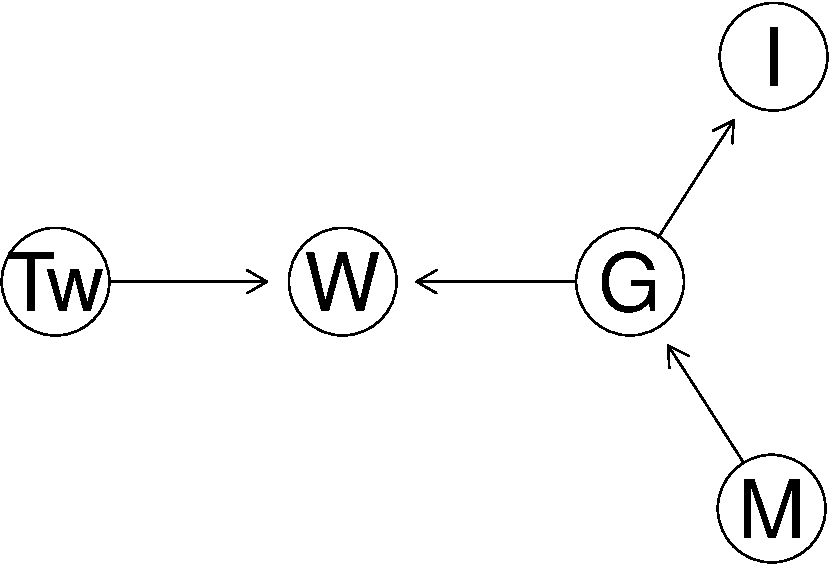
\includegraphics[width=0.7\linewidth]{coherencePaper32_files/figure-latex/unnamed-chunk-9-1} \end{center}
\end{subfigure}} 
\hspace{-1cm}\scalebox{.8}{\begin{subfigure}[!ht]{0.3\textwidth}

\begin{tabular}{lllr}
\toprule
\multicolumn{1}{c}{} & \multicolumn{1}{c}{G} & \multicolumn{1}{c}{Tw} & \multicolumn{1}{c}{} \\
W &  &  & Pr\\
\midrule
1 & 1 & 1 & 0.200\\
0 & 1 & 1 & 0.800\\
1 & 0 & 1 & 0.400\\
0 & 0 & 1 & 0.600\\
1 & 1 & 0 & 0.005\\
0 & 1 & 0 & 0.995\\
1 & 0 & 0 & 0.200\\
0 & 0 & 0 & 0.800\\
\bottomrule
\end{tabular}
\end{subfigure}}
\caption{BN for the \textsf{Dunnit} problem. The key difference for the twin version lies in the construction of the CPT for \textsf{W}. The table gives conditional probabilities for \textsf{W} given various joint states of \textsf{Tw} and \textsf{G}.}
\label{fig:twin}
\end{figure}

\textbf{Results.}
Coherence calculations result in Table \ref{tab:dunnitCoherence} and how they fare with respect to the desideratum is displayed in Table \ref{tab:dunnitDesiderata}.

\begin{table}[H]

\caption{\label{tab:dunnitCoherence}Coherence scores for the Dunnit scenario (rounded).}
\centering
\resizebox{\linewidth}{!}{
\begin{tabular}[t]{lrrrrrrrrrr}
\toprule
  & OG & OGGen & Sh & ShG & DM & R & Fi & SZ & SLR & SL\\
\midrule
\cellcolor{gray!6}{Dunnit: MGWI 1111} & \cellcolor{gray!6}{0} & \cellcolor{gray!6}{0.087} & \cellcolor{gray!6}{4.294} & \cellcolor{gray!6}{11.012} & \cellcolor{gray!6}{0.167} & \cellcolor{gray!6}{0.266} & \cellcolor{gray!6}{0.169} & \cellcolor{gray!6}{-0.891} & \cellcolor{gray!6}{56.689} & \cellcolor{gray!6}{-0.817}\\
Dunnit: MTwGWI 11111 & 0 & 0.042 & 73.836 & 13.669 & 0.150 & 0.214 & 0.385 & 0.267 & 57.002 & 0.451\\
\bottomrule
\end{tabular}}
\end{table}

\begin{table}[H]

\caption{\label{tab:dunnitDesiderata}Desideratum satisfaction for the Dunnit scenario.}
\centering
\resizebox{\linewidth}{!}{
\begin{tabular}[t]{lllllllllll}
\toprule
  & OG & OGGen & Sh & ShG & DM & R & Fi & SZ & SLR & SL\\
\midrule
\cellcolor{gray!6}{Dunnit: Dunnit$<$Twin} & \cellcolor{gray!6}{FALSE} & \cellcolor{gray!6}{FALSE} & \cellcolor{gray!6}{TRUE} & \cellcolor{gray!6}{TRUE} & \cellcolor{gray!6}{FALSE} & \cellcolor{gray!6}{FALSE} & \cellcolor{gray!6}{TRUE} & \cellcolor{gray!6}{TRUE} & \cellcolor{gray!6}{TRUE} & \cellcolor{gray!6}{TRUE}\\
\bottomrule
\end{tabular}}
\end{table}

\hypertarget{japanese-swords}{%
\subsection{Japanese swords}\label{japanese-swords}}

\textbf{The scenario.} The next challenge comes from (Meijs \& Douven, 2007, p. 414):

\begin{quote}
  We start by considering two situations in both of which it is assumed that a murder has been committed in a street in a big city with 10,000,000 inhabitants, 1,059 of them being Japanese, 1,059 of them owning Samurai swords, and 9 of them both being Japanese and owning Samurai swords. In situation I we assume that the murderer lives in the city and that everyone living in the city is equally likely to be the murderer. In situation II, on the other hand, we make the assumption that the victim was murdered by someone living in the street in which her body was found. In that street live 100 persons, 10 of them being Japanese, 10 owning a Samurai sword, and 9 both being Japanese and owning a Samurai sword. [\dots] [In situation III] we have 12 suspects who all live in the same house, and 10 of them are Japanese, 10 own a Samurai sword, and 9 are both Japanese and Samurai sword owners.
\end{quote}

\noindent The nodes involved are as in Table \ref{tab:japanesePropositions1}.

\begin{table}[H]

\caption{\label{tab:japanesePropositions1}Nodes in the Japanese swords scenario.}
\centering
\begin{tabular}[t]{ll}
\toprule
node & content\\
\midrule
\cellcolor{gray!6}{J} & \cellcolor{gray!6}{The murderer is Japanese.}\\
O & The murderer owns a Samurai sword.\\
\bottomrule
\end{tabular}
\end{table}

Now, we look at three separate scenarios: (\textsf{1}) The murderer lives in the city, (\textsf{2}) The murderer lives in the street popular among Japanese owners of Samurai swords, and (\textsf{3}) The murderer lives in the house with many Japanese owners of Samurai swords.

\noindent \textbf{Desiderata.} In all of the above situations the number of Japanese owners of Samurai swords remains the same. However, situations 1 and 2 differ in the relative overlap of \s{J} and \s{O}. Because \s{J} and \s{O} are more correlated in situation 2, it seems more coherent than situation 1.

\vspace{2mm}\begin{description}
    \item[(\s{JO2}$>$\s{JO1})]  \{\s{J,O,2}\} should be more coherent than \{\s{J,O,1}\}.
\end{description}\vspace{2mm}

However, bigger overlap, supposedly, doesn't have to indicate higher coherence. In situation 3 \s{J} and \s{O} confirm each other to a lesser extent than in situation 2 (compare \(P(J|O)-P(J)\) and \(P(O|J)-P(O)\) in both cases), and for this reason Douven and Meijs claim that situation 2 is more coherent than situation 3.
\vspace{2mm}

\begin{description}
    \item[(\s{JO2}$>$\s{JO3})]  \{\s{J,O,2}\} should be more coherent than \{\s{J,O,3}\}.
\end{description}\vspace{2mm}

\noindent We don't have clear intuitions about this desideratum. It seems to be in tension with the requirement offered by Siebel (2004, p. 336) which we'll discuss in the next subsection.\todo{fix when done}

\textbf{Bayesian networks.} There is a common DAG for the three scenarios, but the CPTs differ (Figure \ref{fig:japanese}).

\begin{figure}[H]
\scalebox{0.5}{
\hspace{2.5cm}\begin{subfigure}[!ht]{0.4\textwidth}

\begin{center}
\includegraphics[width=0.7\linewidth]{coherencePaper32_files/figure-latex/unnamed-chunk-13-1} \end{center}
\end{subfigure}} \hfill
\begin{subfigure}[!ht]{0.2\textwidth}

\begin{tabular}{lr}
\toprule
J & Pr\\
\midrule
1 & 0\\
0 & 1\\
\bottomrule
\end{tabular}


\begin{tabular}{lrr}
\toprule
\multicolumn{1}{c}{O} & \multicolumn{2}{c}{J} \\
  & 1 & 0\\
\midrule
1 & 0.008 & 0\\
0 & 0.992 & 1\\
\bottomrule
\end{tabular}
\caption{Scenario 1.}
\end{subfigure} 
\begin{subfigure}[!ht]{0.2\textwidth}

\begin{tabular}{lr}
\toprule
J & Pr\\
\midrule
1 & 0.1\\
0 & 0.9\\
\bottomrule
\end{tabular}


\begin{tabular}{lrr}
\toprule
\multicolumn{1}{c}{O} & \multicolumn{2}{c}{J} \\
  & 1 & 0\\
\midrule
1 & 0.9 & 0.011\\
0 & 0.1 & 0.989\\
\bottomrule
\end{tabular}
\caption{Scenario 2.}
\end{subfigure}  \hfill
\begin{subfigure}[!ht]{0.2\textwidth}

\begin{tabular}{lr}
\toprule
J & Pr\\
\midrule
1 & 0.833\\
0 & 0.167\\
\bottomrule
\end{tabular}


\begin{tabular}{lrr}
\toprule
\multicolumn{1}{c}{O} & \multicolumn{2}{c}{J} \\
  & 1 & 0\\
\midrule
1 & 0.9 & 0.5\\
0 & 0.1 & 0.5\\
\bottomrule
\end{tabular}
\caption{Scenario 3.}
\end{subfigure} 
\caption{A common DAG and three sets of CPTs for the \textsf{Japanese Swords} problem.}
\label{fig:japanese}
\end{figure}

\textbf{Results.} Coherence calculations are in Table \ref{tab:japaneseCoherence} and the status of the desiderata involved is displayed in Table \ref{tab:japaneseDesiderata}.

\begin{table}[H]

\caption{\label{tab:japaneseCoherence}Coherence scores in the Japanese swords scenarios (rounded).}
\centering
\resizebox{\linewidth}{!}{
\begin{tabular}[t]{lrrrrrrrrrr}
\toprule
  & OG & OGGen & Sh & ShG & DM & R & Fi & SZ & SLR & SL\\
\midrule
\cellcolor{gray!6}{Japanese Swords 1: JO 11} & \cellcolor{gray!6}{0.004} & \cellcolor{gray!6}{0.004} & \cellcolor{gray!6}{80.251} & \cellcolor{gray!6}{80.251} & \cellcolor{gray!6}{0.008} & \cellcolor{gray!6}{0.008} & \cellcolor{gray!6}{0.976} & \cellcolor{gray!6}{0.008} & \cellcolor{gray!6}{80.93} & \cellcolor{gray!6}{0.976}\\
Japanese Swords 2: JO 11 & 0.818 & 0.818 & 9.000 & 9.000 & 0.800 & 0.900 & 0.976 & 0.889 & 81.00 & 0.976\\
\cellcolor{gray!6}{Japanese Swords 3: JO 11} & \cellcolor{gray!6}{0.818} & \cellcolor{gray!6}{0.818} & \cellcolor{gray!6}{1.080} & \cellcolor{gray!6}{1.080} & \cellcolor{gray!6}{0.067} & \cellcolor{gray!6}{0.900} & \cellcolor{gray!6}{0.286} & \cellcolor{gray!6}{0.400} & \cellcolor{gray!6}{1.80} & \cellcolor{gray!6}{0.286}\\
\bottomrule
\end{tabular}}
\end{table}

\begin{table}[H]

\caption{\label{tab:japaneseDesiderata}Desiderata satisfaction in the Japanese swords scenarios.}
\centering
\resizebox{\linewidth}{!}{
\begin{tabular}[t]{lllllllllll}
\toprule
  & OG & OGGen & Sh & ShG & DM & R & Fi & SZ & SLR & SL\\
\midrule
\cellcolor{gray!6}{Swords: JO2$>$JO1} & \cellcolor{gray!6}{TRUE} & \cellcolor{gray!6}{TRUE} & \cellcolor{gray!6}{FALSE} & \cellcolor{gray!6}{FALSE} & \cellcolor{gray!6}{TRUE} & \cellcolor{gray!6}{TRUE} & \cellcolor{gray!6}{TRUE} & \cellcolor{gray!6}{TRUE} & \cellcolor{gray!6}{TRUE} & \cellcolor{gray!6}{TRUE}\\
Swords: JO2$>$JO3 & FALSE & FALSE & TRUE & TRUE & TRUE & FALSE & TRUE & TRUE & TRUE & TRUE\\
\bottomrule
\end{tabular}}
\end{table}

\hypertarget{robbers}{%
\subsection{Robbers}\label{robbers}}

\textbf{The scenario.} A challenge put forward by Siebel (2004, p. 336) goes as follows:

\begin{quote}
    Let there be ten equiprobable suspects for a murder. All of them previously committed at least one crime, two a robbery, two pick-pocketing, and the remaining six both crimes. There is thus a substantial overlap: of the total of eight suspects who committed a robbery, six were also involved in pick-pocketing, and conversely. 
\end{quote}

\noindent The nodes involved are Table \ref{tab:robbersPropositions}.

\begin{table}[H]

\caption{\label{tab:robbersPropositions}Nodes in the Robbers scenario.}
\centering
\begin{tabular}[t]{ll}
\toprule
node & content\\
\midrule
\cellcolor{gray!6}{W} & \cellcolor{gray!6}{Real perpetrator status (three possible states).}\\
P & The murderer is a pickpocket.\\
\cellcolor{gray!6}{R} & \cellcolor{gray!6}{The murderer is a robber.}\\
\bottomrule
\end{tabular}
\end{table}

\noindent  \textbf{Desiderata.} The first observation is that the set of propositions that corresponds to the situation in which a murderer committed both crimes should be regarded coherent. Most suspects committed both crimes, so this option is even the most probable one.
\vspace{2mm}

\begin{description}
    \item[(\s{PR}\textgreater \s{neutral})] \{\s{P,R}\} should be regarded coherent. 
\end{description}\vspace{2mm}

According to Siebel (2004, p. 336) committing both crimes by the murderer should also be regarded more coherent than committing only one crime.
\vspace{2mm}

\begin{description}
    \item[(\s{PR}$>$\s{P}$\neg$\s{R})] \{\s{P,R}\} should be more coherent than \{\s{P},$\neg$\s{R}\} and \{$\neg$\s{P},\s{R}\}.
\end{description}\vspace{2mm}

\noindent  This requirement is slightly more controversial. Even though \{\s{P,R}\} is the most probable setup, \s{P} and \s{R} disconfirm each other (\(Pr(P|R)<Pr(P)\) and \(Pr(R|P)<Pr(R)\)). Moreover, the intuition behind this desideratum seems to conflict with the intuition behind (\s{JO2}\(>\)\s{JO3}).

\textbf{Bayesian networks.} The robbers counterexample involves a phenomenon we've already seen: it is not clear whether the information about the prior probabilities is supposed to be part of the narration or not. \todo{is this comment still needed?} If we want to include this information in our coherence assessment, we can do this employing a single BN.

\vspace{1mm}
\footnotesize

\normalsize

\begin{figure}[H]
\begin{subfigure}[!ht]{0.4\textwidth}

\begin{center}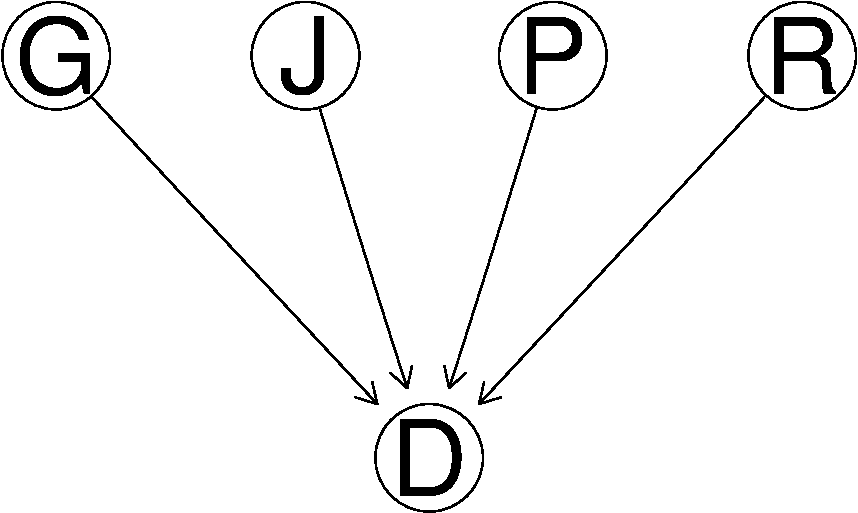
\includegraphics{coherencePaper32_files/figure-latex/unnamed-chunk-20-1} \end{center}
\end{subfigure} \hfill
\begin{subfigure}[!ht]{0.4\textwidth}

\centering\begingroup\fontsize{9}{11}\selectfont
\begin{tabular}{lr}
\toprule
  & Pr\\
\midrule
\cellcolor{gray!6}{OnlyP} & \cellcolor{gray!6}{0.2}\\
OnlyR & 0.2\\
\cellcolor{gray!6}{Both} & \cellcolor{gray!6}{0.6}\\
\bottomrule
\end{tabular}




\begin{tabular}{lrrr}
\toprule
\multicolumn{1}{c}{MisP} & \multicolumn{3}{c}{WhoMurdered} \\
  & OnlyP & OnlyR & Both\\
\midrule
\cellcolor{gray!6}{1} & \cellcolor{gray!6}{1} & \cellcolor{gray!6}{0} & \cellcolor{gray!6}{1}\\
0 & 0 & 1 & 0\\
\bottomrule
\end{tabular}

\begin{tabular}{lrrr}
\toprule
\multicolumn{1}{c}{MisR} & \multicolumn{3}{c}{WhoMurdered} \\
  & OnlyP & OnlyR & Both\\
\midrule
\cellcolor{gray!6}{1} & \cellcolor{gray!6}{0} & \cellcolor{gray!6}{1} & \cellcolor{gray!6}{1}\\
0 & 1 & 0 & 0\\
\bottomrule
\end{tabular}


\endgroup{}


\end{subfigure}
\caption{BN for the \textsf{Robbers} problem.}
\label{fig:Robbers}
\end{figure}

\textbf{Results.} Coherence calculations yield the results in Table \ref{tab:robbersCoherence}, and the performance of the coherence measures with respect to the desiderata is illustrated in Table \ref{tab:robbersDesiderata}.

\begin{table}[H]

\caption{\label{tab:robbersCoherence}Coherence scores in the Robbers scenario (rounded).}
\centering
\resizebox{\linewidth}{!}{
\begin{tabular}[t]{lrrrrrrrrrr}
\toprule
  & OG & OGGen & Sh & ShG & DM & R & Fi & SZ & SLR & SL\\
\midrule
Robbers: MIsPMIsR 11 & 0.60 & 0.60 & 0.937 & 0.937 & -0.050 & 0.750 & -0.143 & 0.60 & Inf & 0.60\\
Robbers: MIsPMIsR 10 & 0.25 & 0.25 & 1.250 & 1.250 & 0.125 & 0.625 & 0.571 & -0.36 & Inf & -0.36\\
Robbers: MIsPMIsR 01 & 0.25 & 0.25 & 1.250 & 1.250 & 0.125 & 0.625 & 0.571 & -0.36 & Inf & -0.36\\
\bottomrule
\end{tabular}}
\end{table}

\begin{table}[H]

\caption{\label{tab:robbersDesiderata}Desiderata satisfaction in the Robbers problem.}
\centering
\resizebox{\linewidth}{!}{
\begin{tabular}[t]{lllllllllll}
\toprule
  & OG & OGGen & Sh & ShG & DM & R & Fi & SZ & SLR & SL\\
\midrule
Robbers: PR$>$P$\neg$R & TRUE & TRUE & FALSE & FALSE & FALSE & TRUE & FALSE & TRUE & FALSE & TRUE\\
Robbers: PR$>$neutral & NA & NA & FALSE & FALSE & FALSE & TRUE & FALSE & TRUE & TRUE & TRUE\\
\bottomrule
\end{tabular}}
\end{table}

\hypertarget{the-beatles}{%
\subsection{The Beatles}\label{the-beatles}}

\todo{Consider moving to top of the list.}

\textbf{The scenario.} The challenge has been offered by Shogenji (1999, p. 339) to criticize defining coherence in terms of pairwise coherence --- it shows there are jointly incoherent pairwise coherent sets. The scenario consists of the claims displayed in Table \ref{tab:beatles}.

\begin{table}[H]

\caption{\label{tab:beatles}Nodes in the Beatles scenario.}
\centering
\begin{tabular}[t]{ll}
\toprule
node & content\\
\midrule
\cellcolor{gray!6}{D} & \cellcolor{gray!6}{Exactly one of the Beatles (John, Paul, George and Ringo) is dead.}\\
J & John is alive.\\
\cellcolor{gray!6}{P} & \cellcolor{gray!6}{Paul is alive.}\\
G & George is alive.\\
\cellcolor{gray!6}{R} & \cellcolor{gray!6}{Ringo is alive.}\\
\bottomrule
\end{tabular}
\end{table}

\noindent  \textbf{Desiderata.} The set consisting of all of these propositions is logically inconsistent (even though the propositions are pairwise consistent), so it seems quite intuitive that it should be incoherent.
\vspace{2mm}

\begin{description}
    \item[(below neutral)] \{\s{D,J,P,G,R}\} should be incoherent.
\end{description}\vspace{2mm}

We can make this desideratum a bit stronger by requiring that the coherence score for \{\s{D,J,P,G,R}\} should be minimal.
\vspace{2mm}

\begin{description}
    \item[(minimal)] \{\s{D,J,P,G,R}\} should get the lowest possible coherence value.
\end{description}\vspace{2mm}

\noindent  One may argue that some coherence measures also measure the degree of incoherence, therefore logically inconsistent sets don't need to get the minimal score. We'll discuss this issue further in Section \ref{sec:mean}.\todo{check ref}

For the sake of example, we assume the prior probability of each individual band member being dead to 0.5 (as in the above table), and the CPT for \textsf{D} is many-dimensional and so difficult to present concisely, but the method is straightforward: probability 1 is given to \textsf{D} in all combinations of the parents in which exactly one is true, and otherwise \textsf{D} gets conditional probability 0.

\begin{figure}[H]
\scalebox{1.6}{
\begin{subfigure}[!ht]{0.3\textwidth}

\begin{center}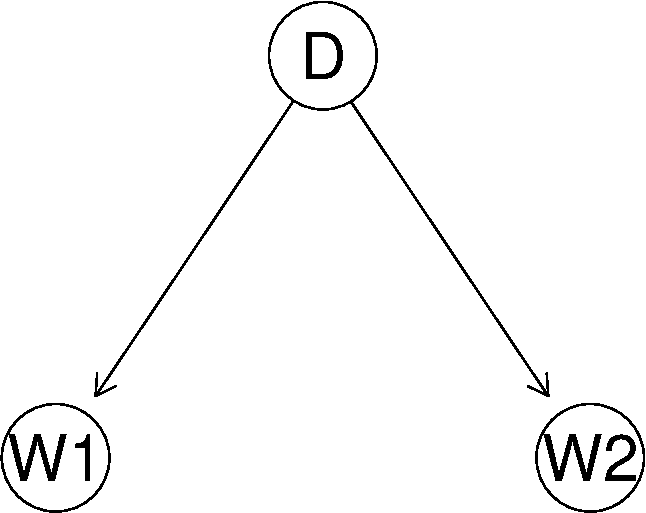
\includegraphics[width=0.7\linewidth]{coherencePaper32_files/figure-latex/unnamed-chunk-23-1} \end{center}
\end{subfigure}} \hfill
\begin{subfigure}[!ht]{0.2\textwidth}

\begin{tabular}{lr}
\toprule
G & Pr\\
\midrule
1 & 0.5\\
0 & 0.5\\
\bottomrule
\end{tabular}
\end{subfigure}
\caption{Bayesian network for the \textsf{Beatles} scenario.}
\end{figure}

\textbf{Results.} Coherence calculations give the results from Table \ref{tab:beatlesCoherence}, and the satisfaction of the desiderata involved can be inspected by looking at Table \ref{tab:beatlesDesiderata}.

\begin{table}[H]

\caption{\label{tab:beatlesCoherence}Coherence scores in the Beatles scenario (rounded).}
\centering
\resizebox{\linewidth}{!}{
\begin{tabular}[t]{lrrrrrrrrrr}
\toprule
  & OG & OGGen & Sh & ShG & DM & R & Fi & SZ & SLR & SL\\
\midrule
\cellcolor{gray!6}{Beatles: JPGRD 11111} & \cellcolor{gray!6}{0} & \cellcolor{gray!6}{0.202} & \cellcolor{gray!6}{0} & \cellcolor{gray!6}{1.423} & \cellcolor{gray!6}{0.025} & \cellcolor{gray!6}{0.322} & \cellcolor{gray!6}{-0.036} & \cellcolor{gray!6}{-1} & \cellcolor{gray!6}{0} & \cellcolor{gray!6}{-1}\\
\bottomrule
\end{tabular}}
\end{table}

\begin{table}[H]

\caption{\label{tab:beatlesDesiderata}Desiderata satisfaction in the Beatles scenario.}
\centering
\resizebox{\linewidth}{!}{
\begin{tabular}[t]{lllllllllll}
\toprule
  & OG & OGGen & Sh & ShG & DM & R & Fi & SZ & SLR & SL\\
\midrule
\cellcolor{gray!6}{Beatles: below neutral} & \cellcolor{gray!6}{NA} & \cellcolor{gray!6}{NA} & \cellcolor{gray!6}{TRUE} & \cellcolor{gray!6}{FALSE} & \cellcolor{gray!6}{FALSE} & \cellcolor{gray!6}{FALSE} & \cellcolor{gray!6}{TRUE} & \cellcolor{gray!6}{TRUE} & \cellcolor{gray!6}{TRUE} & \cellcolor{gray!6}{TRUE}\\
Beatles: minimal & TRUE & FALSE & TRUE & FALSE & FALSE & FALSE & FALSE & TRUE & TRUE & TRUE\\
\bottomrule
\end{tabular}}
\end{table}

\hypertarget{the-witnesses}{%
\subsection{The Witnesses}\label{the-witnesses}}

\textbf{The scenario.}This one comes from (Olsson, 2005, p. 391). Again, equally reliable witnesses try to identify a criminal. Consider the reports listed in Table \ref{tab:witnessesProp} (we extended the original scenario by adding \s{W5}).

\begin{table}[H]

\caption{\label{tab:witnessesProp}Testimonies in the Witnesses scenario.}
\centering
\begin{tabular}[t]{ll}
\toprule
node & content\\
\midrule
\cellcolor{gray!6}{W1} & \cellcolor{gray!6}{Witness no. 1: ‘‘Steve did it’’}\\
W2 & Witness no. 2: ‘‘Steve did it’’\\
\cellcolor{gray!6}{W3} & \cellcolor{gray!6}{Witness no. 3: ‘‘Steve, Martin or David did it’’}\\
W4 & Witness no. 4: ‘‘Steve, John or James did it’’\\
\cellcolor{gray!6}{W5} & \cellcolor{gray!6}{Wittness no. 5: ‘‘Steve, John or Peter did it’’}\\
D & Who committed the deed (6  possible values)\\
\bottomrule
\end{tabular}
\end{table}

\noindent Note that this time each proposition has the structure ``Witness no. \(X\) claims that \dots'' instead of explicitly stating the witness' testimony.

\textbf{Desiderata.} First, we can observe that \s{W1} and \s{W2} fully agree. Testimonies of \s{W3} and \s{W4} overlap only partially, therefore it seems that \{\s{W1},\s{W2}\} is more coherent than \{\s{W3},\s{W4}\}.
\vspace{2mm}

\begin{description}
    \item[(\s{W1W2\textgreater W3W4})] \{\s{W1},\s{W2}\} should be more coherent than \{\s{W3},\s{W4}\}.
\end{description}\vspace{2mm}

Similarly, there is a greater agreement between \s{W4} and \s{W5} than \s{W3} and \s{W4}, so \{\s{W4},\s{W5}\} seems more coherent than \{\s{W3},\s{W4}\}.
\vspace{2mm}

\begin{description}
    \item[(\s{W4W5\textgreater W3W4})] \{\s{W4},\s{W5}\} should be more coherent than \{\s{W3},\s{W4}\}.
\end{description}\vspace{2mm}

\textbf{Bayesian networks.} Two requirements are associated with this example: both \(\{\)\textsf{W1, W2}\(\}\) and \(\{\)\textsf{W4, W5}\(\}\) should be more coherent than \(\{\)\textsf{W3, W4}\(\}\). The basic idea behind the CPTs we used is that for any particular witness we take the probability of them including the perpetrator in their list to be 0.8, and the probability of including an innocent to be .05. Of course, the example can be run with different conditional probability tables. Let's first take a look at the BN for the first scenario (Figure \ref{fig:w1w2}).

\vspace{1mm}
\footnotesize

\normalsize

\begin{figure}[H]
\scalebox{1.2}{
\hspace{1cm}\begin{subfigure}[!ht]{0.4\textwidth}

\begin{center}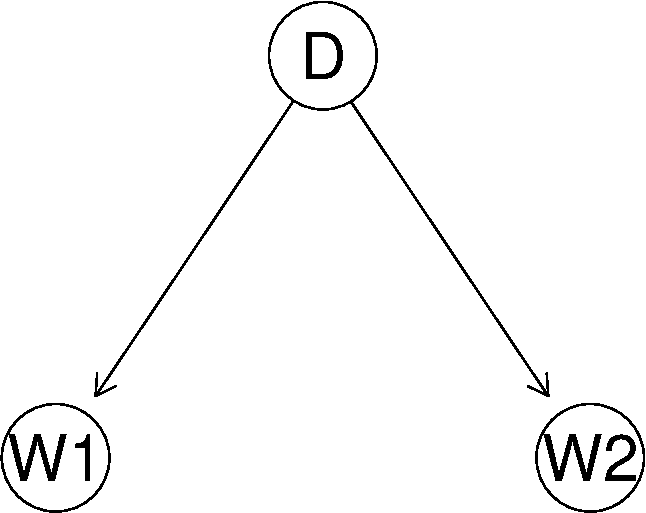
\includegraphics[width=1\linewidth]{coherencePaper32_files/figure-latex/unnamed-chunk-28-1} \end{center}
\end{subfigure}} \hfill
\begin{subfigure}[!ht]{0.3\textwidth}
\begin{tabular}{lr}
\toprule
D & Pr\\
\midrule
\cellcolor{gray!6}{Steve} & \cellcolor{gray!6}{0.167}\\
Martin & 0.167\\
\cellcolor{gray!6}{David} & \cellcolor{gray!6}{0.167}\\
John & 0.167\\
\cellcolor{gray!6}{James} & \cellcolor{gray!6}{0.167}\\
Peter & 0.167\\
\bottomrule
\end{tabular}
\end{subfigure}
\centering
\begin{subfigure}[!ht]{0.3\textwidth}
\begin{tabular}{lrrrrrr}
\toprule
\multicolumn{1}{c}{W1} & \multicolumn{2}{c}{D} \\
  & Steve & Martin & David & John & James & Peter\\
\midrule
\cellcolor{gray!6}{1} & \cellcolor{gray!6}{0.8} & \cellcolor{gray!6}{0.05} & \cellcolor{gray!6}{0.05} & \cellcolor{gray!6}{0.05} & \cellcolor{gray!6}{0.05} & \cellcolor{gray!6}{0.05}\\
0 & 0.2 & 0.95 & 0.95 & 0.95 & 0.95 & 0.95\\
\bottomrule
\end{tabular}
\end{subfigure}
\caption{BN for the \textsf{W1W2} narration in the \textsf{Witness} problem. CPT for \textsf{W2} is identical to the one for \textsf{W1}.}
\label{fig:w1w2}
\end{figure}

The CPT for \textsf{D} is uniform. The table for \textsf{W1} provides the conditional probability of \textsf{W1} listing (\textsf{W1}=1) or not listing (\textsf{W1}=0) a particular person given that the actual value of \textsf{D} is Steve/Martin/\dots. The underlying rule is: if someone is guilty, a witness will mention them with probability \(.8\), and if they aren't, they will be listed with probability \(.05\). In the remaining two BNs for the problem the CPT for \textsf{D} remains the same, and the CPTs for the witness nodes are analogous to the one for \textsf{W1}. The remaining BNs have the following obvious DAGs (Fig. \ref{fig:witness}).

\begin{figure}[H]
\centering
\scalebox{1.2}{
\begin{subfigure}[!ht]{0.4\textwidth}

\begin{center}
\includegraphics[width=1\linewidth]{coherencePaper32_files/figure-latex/unnamed-chunk-29-1} \end{center}
\end{subfigure}}

\scalebox{1.2}{\begin{subfigure}[!ht]{0.4\textwidth}

\begin{center}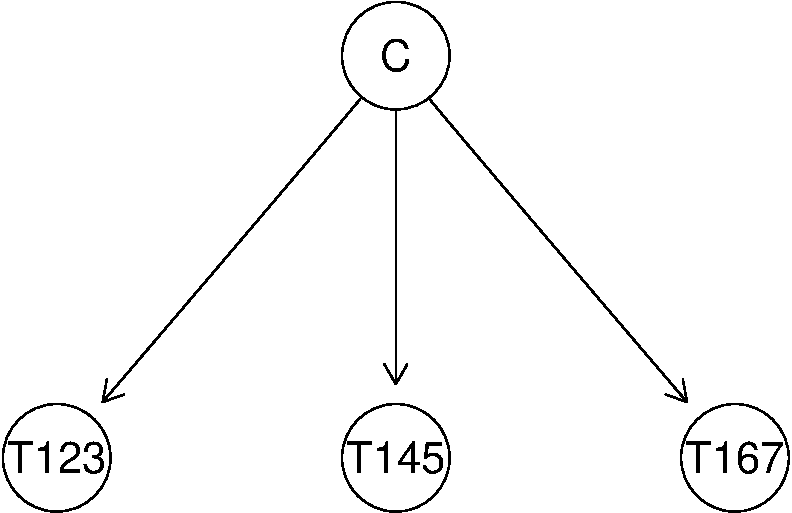
\includegraphics[width=1\linewidth]{coherencePaper32_files/figure-latex/unnamed-chunk-30-1} \end{center}
\end{subfigure}}
\caption{Two remaining DAGs for the \textsf{Witness} problem.}
\label{fig:witness}
\end{figure}

\textbf{Results.} We think that what this example illustrates is that we should really carefully think about whose cognitive perspective is taken when we represent a narration using a BN, focusing on whether the BN involves nodes which are not part of the narration whose coherence is to be evaluated. In particular, the probabilistic information about the uniform distribution of guilt probability is not part of any of the three involved narrations, but rather a part of a third-person set-up prior to obtaining any evidence.

To evaluate the coherence of a narration, at least for unmentioned assumptions that one doesn't have strong independent reasons to keep, one should think counterfactually, granting the consequences of the narration and asking what would happen if it indeed was true. In our case, a judge who evaluates the coherence of witness testimonies once she has heard them, no longer thinks that the distribution of \textsf{D} is uniform. And this agrees with the counterfactual strategy we just described: it is a consequence of the probabilistic set-up and the content of \textsf{W1} and \textsf{W2} that if \textsf{W1} and \textsf{W2} were true, the distribution for \textsf{D} no longer would be uniform, and so it is unfair to judge the coherence of this scenario without giving up this assumption and updating one's assumptions about \textsf{D}.

In such a case, we think, we should update \textsf{D} to what it would be had \textsf{W1} and \textsf{W2} be instantiated with 1s and use these updated probabilities to build the weights used in our coherence calculations for this narration (and proceed accordingly, instead updating on another set of narration nodes in the coherence evaluation of other narrations).\footnote{Note  however that  you should not simply instantiate the BN with \textsf{W1} and \textsf{W2}, propagate and run the coherence calculations on the updated BN. Then both these nodes would get 1s in their respective CPTs and coherence calculations would make   all  confirmation measures involved in such calculations  based on posterior probability equal 1 (Table \\ref{witnessesWeights}). If narration members have probability one, no other information will be able to confirm it.}

\begin{table}[H]

\caption{\label{tab:witnessesWeights}Propagated probabilities for D in the Witnesses scenario (rounded).}
\centering
\begin{tabular}[t]{lrrrrrr}
\toprule
  & Steve & Martin & David & John & James & Peter\\
\midrule
\cellcolor{gray!6}{Pr} & \cellcolor{gray!6}{0.981} & \cellcolor{gray!6}{0.004} & \cellcolor{gray!6}{0.004} & \cellcolor{gray!6}{0.004} & \cellcolor{gray!6}{0.004} & \cellcolor{gray!6}{0.004}\\
\bottomrule
\end{tabular}
\end{table}

Once this strategy is taken, the problem turns out to be not that challenging for any of the coherence measures under discussion. The coherence scores are displayed in Table \ref{tab:witnessesCoherence} and the status of the desiderata is in Table \ref{tab:witnessesDesiderata}. Now all the weights come from Bayesian networks updated from the perspertive of a given narration, which is emphasized by our use of abbreviations SZnarr, SLRnarr, and SLnarr.

\begin{table}[H]

\caption{\label{tab:witnessesCoherence}Coherence scores in the Witnesses scenario (rounded).}
\centering
\resizebox{\linewidth}{!}{
\begin{tabular}[t]{lrrrrrrrrrr}
\toprule
  & OG & OGGen & Sh & ShGen & DM & R & Fi & SZnarr & SLRnarr & SLnarr\\
\midrule
\cellcolor{gray!6}{Witness: W1W2 11} & \cellcolor{gray!6}{0.451} & \cellcolor{gray!6}{0.451} & \cellcolor{gray!6}{3.551} & \cellcolor{gray!6}{3.551} & \cellcolor{gray!6}{0.446} & \cellcolor{gray!6}{0.621} & \cellcolor{gray!6}{0.771} & \cellcolor{gray!6}{0.729} & \cellcolor{gray!6}{18.501} & \cellcolor{gray!6}{0.871}\\
Witness: W3W4 11 & 0.187 & 0.187 & 0.740 & 0.740 & -0.110 & 0.315 & -0.234 & 0.494 & 4.863 & 0.528\\
\cellcolor{gray!6}{Witness: W4W5 11} & \cellcolor{gray!6}{0.365} & \cellcolor{gray!6}{0.365} & \cellcolor{gray!6}{1.260} & \cellcolor{gray!6}{1.260} & \cellcolor{gray!6}{0.110} & \cellcolor{gray!6}{0.535} & \cellcolor{gray!6}{0.218} & \cellcolor{gray!6}{0.602} & \cellcolor{gray!6}{5.236} & \cellcolor{gray!6}{0.637}\\
\bottomrule
\end{tabular}}
\end{table}

\begin{table}[H]

\caption{\label{tab:witnessesDesiderata}Desiderata satisfaction in the Witnesses scenario.}
\centering
\resizebox{\linewidth}{!}{
\begin{tabular}[t]{lllllllllll}
\toprule
  & OG & OGGen & Sh & ShGen & DM & R & Fi & SZnarr & SLRnarr & SLnarr\\
\midrule
\cellcolor{gray!6}{Witness: W$_1$W$_2>$W$_3$W$_4$} & \cellcolor{gray!6}{TRUE} & \cellcolor{gray!6}{TRUE} & \cellcolor{gray!6}{TRUE} & \cellcolor{gray!6}{TRUE} & \cellcolor{gray!6}{TRUE} & \cellcolor{gray!6}{TRUE} & \cellcolor{gray!6}{TRUE} & \cellcolor{gray!6}{TRUE} & \cellcolor{gray!6}{TRUE} & \cellcolor{gray!6}{TRUE}\\
Witness: W$_4$W$_5>$W$_3$W$_4$ & TRUE & TRUE & TRUE & TRUE & TRUE & TRUE & TRUE & TRUE & TRUE & TRUE\\
\bottomrule
\end{tabular}}
\end{table}

\hypertarget{depth}{%
\subsection{Depth}\label{depth}}

\textbf{The scenario.} There are eight equally likely suspects \(1, \dots, 8\), and three equally reliable witnesses \(a, b, c\), each trying to identify the person responsible for the crime. Compare two different situations -- \s{X1} and \s{X2}:
\begin{align*}
    X_1 & = \{a:(1 \vee 2 \vee 3), b:(1\vee 2 \vee 4), c:(1 \vee 3 \vee 4)\}\\
    X_2 & =  \{a:(1 \vee 2 \vee 3), b:(1\vee  4 \vee 5), c:(1 \vee 6 \vee 7)\}
\end{align*}

\noindent \textbf{Desiderata.} In \s{X1} witnesses' testimonies have bigger overlap, between each pair of the witnesses 2 suspects are the same, and in \s{X2} only 1 suspect is always the same. Following Schupbach (2008), one may have an intuition that the first situation is more coherent.
\vspace{2mm}

\begin{description}
    \item[(\s{X1\textgreater X2})] $X_1$  should be more coherent than $X_2$.
\end{description}\vspace{2mm}

\noindent \textbf{Bayesian networks.} We start with representing the two scenarios with two fairly natural BNs (\textsf{C} stands for who Committed the crime, \textsf{TXYZ} stands for Testimony that \(X\vee Y \vee Z\)), see Figures \ref{fig:dod1} and \ref{fig:dod2}.

\begin{figure}[H]
\scalebox{1.7}{
\begin{subfigure}[!ht]{0.4\textwidth}

\begin{center}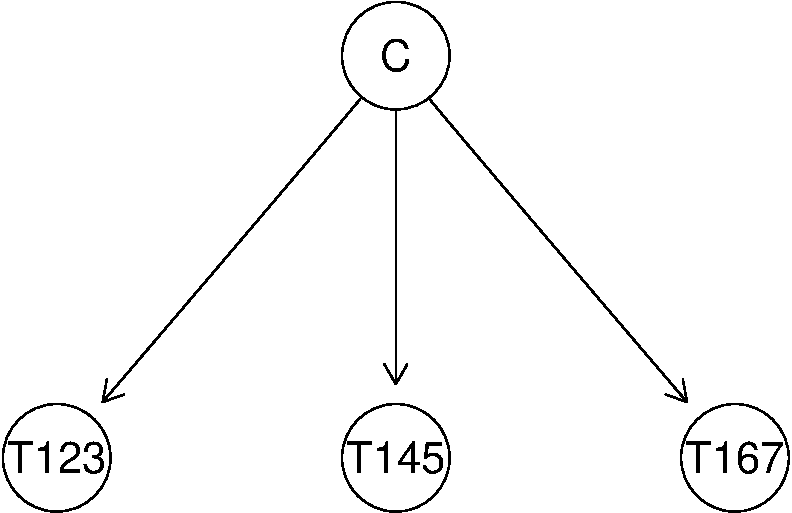
\includegraphics[width=0.7\linewidth]{coherencePaper32_files/figure-latex/unnamed-chunk-33-1} \end{center}
\end{subfigure}} 
\hspace{-1cm}\scalebox{0.6}{\begin{subfigure}[!ht]{0.3\textwidth}

\begin{tabular}{lr}
\toprule
C & Pr\\
\midrule
1 & 0.125\\
2 & 0.125\\
3 & 0.125\\
4 & 0.125\\
5 & 0.125\\
6 & 0.125\\
7 & 0.125\\
8 & 0.125\\
\bottomrule
\end{tabular}


\begin{tabular}{lrrrrrrrr}
\toprule
\multicolumn{1}{c}{T123} & \multicolumn{2}{c}{C} \\
  & 1 & 2 & 3 & 4 & 5 & 6 & 7 & 8\\
\midrule
1 & 1 & 1 & 1 & 0 & 0 & 0 & 0 & 0\\
0 & 0 & 0 & 0 & 1 & 1 & 1 & 1 & 1\\
\bottomrule
\end{tabular}


\begin{tabular}{lrrrrrrrr}
\toprule
\multicolumn{1}{c}{T124} & \multicolumn{2}{c}{C} \\
  & 1 & 2 & 3 & 4 & 5 & 6 & 7 & 8\\
\midrule
1 & 1 & 1 & 0 & 1 & 0 & 0 & 0 & 0\\
0 & 0 & 0 & 1 & 0 & 1 & 1 & 1 & 1\\
\bottomrule
\end{tabular}


\begin{tabular}{lrrrrrrrr}
\toprule
\multicolumn{1}{c}{T134} & \multicolumn{2}{c}{C} \\
  & 1 & 2 & 3 & 4 & 5 & 6 & 7 & 8\\
\midrule
1 & 1 & 0 & 1 & 1 & 0 & 0 & 0 & 0\\
0 & 0 & 1 & 0 & 0 & 1 & 1 & 1 & 1\\
\bottomrule
\end{tabular}
\end{subfigure}}
\caption{BN for \textsf{X1} in the \textsf{Depth} problem.}
\label{fig:dod1}
\end{figure}

\begin{figure}[H]
\scalebox{1.7}{
\begin{subfigure}[!ht]{0.4\textwidth}

\begin{center}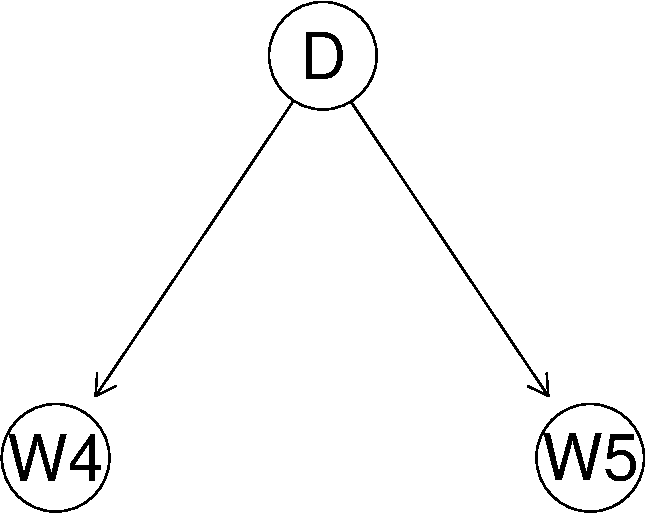
\includegraphics[width=0.7\linewidth]{coherencePaper32_files/figure-latex/unnamed-chunk-35-1} \end{center}
\end{subfigure}} 
\hspace{-1cm}\scalebox{0.6}{\begin{subfigure}[!ht]{0.3\textwidth}

\begin{tabular}{lr}
\toprule
C & Pr\\
\midrule
1 & 0.125\\
2 & 0.125\\
3 & 0.125\\
4 & 0.125\\
5 & 0.125\\
6 & 0.125\\
7 & 0.125\\
8 & 0.125\\
\bottomrule
\end{tabular}


\begin{tabular}{lrrrrrrrr}
\toprule
\multicolumn{1}{c}{T123} & \multicolumn{2}{c}{C} \\
  & 1 & 2 & 3 & 4 & 5 & 6 & 7 & 8\\
\midrule
1 & 1 & 1 & 1 & 0 & 0 & 0 & 0 & 0\\
0 & 0 & 0 & 0 & 1 & 1 & 1 & 1 & 1\\
\bottomrule
\end{tabular}


\begin{tabular}{lrrrrrrrr}
\toprule
\multicolumn{1}{c}{T145} & \multicolumn{2}{c}{C} \\
  & 1 & 2 & 3 & 4 & 5 & 6 & 7 & 8\\
\midrule
1 & 1 & 0 & 0 & 1 & 1 & 0 & 0 & 0\\
0 & 0 & 1 & 1 & 0 & 0 & 1 & 1 & 1\\
\bottomrule
\end{tabular}


\begin{tabular}{lrrrrrrrr}
\toprule
\multicolumn{1}{c}{T167} & \multicolumn{2}{c}{C} \\
  & 1 & 2 & 3 & 4 & 5 & 6 & 7 & 8\\
\midrule
1 & 1 & 0 & 0 & 0 & 0 & 1 & 1 & 0\\
0 & 0 & 1 & 1 & 1 & 1 & 0 & 0 & 1\\
\bottomrule
\end{tabular}
\end{subfigure}}
\caption{BN for \textsf{X2} in the \textsf{Depth} problem.}
\label{fig:dod2}
\end{figure}

\textbf{Results.} One effect of dropping the ``the witness testified that'' and using the testimony contents themselves is that the CPTs for the narration nodes are deterministically connected with the root node. In result, the coherence calculations give the results in Table \ref{tab:depthCoherence}, and the status of the desiderata is pictured in Table \ref{tab:depthDesiderata}.

\begin{table}[H]

\caption{\label{tab:depthCoherence}Coherence scores for the Depth problem (rounded).}
\centering
\resizebox{\linewidth}{!}{
\begin{tabular}[t]{lrrrrrrrrrr}
\toprule
  & OG & OGGen & Sh & ShGen & DM & R & Fi & SZ & SLR & SL\\
\midrule
\cellcolor{gray!6}{Depth: T123T124T134 111} & \cellcolor{gray!6}{0.250} & \cellcolor{gray!6}{0.438} & \cellcolor{gray!6}{2.37} & \cellcolor{gray!6}{1.926} & \cellcolor{gray!6}{0.198} & \cellcolor{gray!6}{0.542} & \cellcolor{gray!6}{0.382} & \cellcolor{gray!6}{-0.25} & \cellcolor{gray!6}{Inf} & \cellcolor{gray!6}{-0.25}\\
Depth: T123T145T167 111 & 0.143 & 0.186 & 2.37 & 1.259 & 0.188 & 0.500 & 0.343 & -0.25 & Inf & -0.25\\
\bottomrule
\end{tabular}}
\end{table}

\begin{table}[H]

\caption{\label{tab:depthDesiderata}Desiderata satisfaction for the Depth problem.}
\centering
\resizebox{\linewidth}{!}{
\begin{tabular}[t]{lllllllllll}
\toprule
  & OG & OGGen & Sh & ShGen & DM & R & Fi & SZ & SLR & SL\\
\midrule
\cellcolor{gray!6}{Depth: X$_1>$X$_2$} & \cellcolor{gray!6}{TRUE} & \cellcolor{gray!6}{TRUE} & \cellcolor{gray!6}{FALSE} & \cellcolor{gray!6}{TRUE} & \cellcolor{gray!6}{TRUE} & \cellcolor{gray!6}{TRUE} & \cellcolor{gray!6}{TRUE} & \cellcolor{gray!6}{FALSE} & \cellcolor{gray!6}{FALSE} & \cellcolor{gray!6}{FALSE}\\
\bottomrule
\end{tabular}}
\end{table}

\todo{need to revise this}

Note that this time we listed two values for our measure. \textsf{Structured 1} shows the values obtained if we do not update the weighting of the node not included in the narration, and \textsf{Structured 2} is the result of such an updated weighing (analogous to the updating involved in the \textsf{Witness} problem). Now, what are we to make of this?

\textsf{Structured 1} is negative. This isn't too surprising: after all, this is the coherence of the narration with the probabilistic assumption that the distribution for \textsf{C} is uniform, and this probabilistic assumption undermines the narration. Why, however, does \textsf{Structured 2} equal 1, and why are the results identical for both narrations? This, upon reflection, isn't too suprising either. If the BN and the narration is supposed to represent a single agent's credal state, there is only one state of \textsf{C} in which the whole narration \(X_1\) is true -- trivially, it is the one in which suspect 1 is guilty, and it is the same unique state of \textsf{C} in which the whole narration \(X_2\) is true. Since seen as narrations these sets have exactly the same truth conditions, there is no surprise in them being equally coherent.

What if the sentences in the set are not claims made by one agent and there is no single underlying credal state? We aren't convinced that our tool is optimal for measuring the agreement of multiple witnesses. Instead, there already exists a working measure of such an agreement --- Cohen's \(\kappa\) -- which already gives the desired results.

To illustrate, let's think of a simplified situation (devoid of three-dimensional tables) with two witnesses \(w1\) and \(w2\), where the respective sets are
\(A = \{1 \vee 2 \vee 3, 1\vee 2 \vee 4\}\) and
\(B = \{1 \vee 2 \vee 3, 1\vee 4 \vee 5\}\) and in each set the first proposition comes from \(w1\) and the second from \(w2\). The information for these two sets is pictured in Tables \ref{tab:AkableTab} and \ref{tab:BkableTab}.

\begin{table}[H]

\caption{\label{tab:AkableTab}Situation A in the Depth problem.}
\centering
\begin{tabular}[t]{lrr}
\toprule
  & w2: suspect & w2: innocent\\
\midrule
\cellcolor{gray!6}{w1:suspect} & \cellcolor{gray!6}{2} & \cellcolor{gray!6}{1}\\
w1: innocent & 1 & 4\\
\bottomrule
\end{tabular}
\end{table}

\begin{table}[H]

\caption{\label{tab:BkableTab}Situation B in the Depth problem.}
\centering
\begin{tabular}[t]{lrr}
\toprule
  & w2: suspect & w2: innocent\\
\midrule
\cellcolor{gray!6}{w1: suspect} & \cellcolor{gray!6}{1} & \cellcolor{gray!6}{2}\\
w1: innocent & 2 & 3\\
\bottomrule
\end{tabular}
\end{table}

\noindent Standard calculations using the \textsf{vcd} package results in the unweighted values of Cohen's \(\kappa\) pictured in Table \ref{tab:kappas2table}.

\begin{table}[H]

\caption{\label{tab:kappas2table}Kappas for the Depth scenario.}
\centering
\begin{tabular}[t]{lrr}
\toprule
  & A & B\\
\midrule
\cellcolor{gray!6}{value} & \cellcolor{gray!6}{0.467} & \cellcolor{gray!6}{-0.067}\\
\bottomrule
\end{tabular}
\end{table}

Let's further illustrate our point about the requirement that the BN should represent a single agent's cognitive state. For instance, you can represent, the situation in \(A\) from the perspective of the first witness. This suggests we should focus only on the nodes involved in the narration, and on the fact that from the witness' perspective the suspects are not equally likely. The example doesn't provide us enough information to build a table for \textsf{C}. In fact, no information about the wintess attitude towards this node is given, but given they say what they say, it's unlikely they think the distribution is uniform. So let's take one of the witness' own statements as the root (which ones we choose doesn't change the outcome). Clearly (or, at least, hopefully, if we talk about witnesses), the agent thinks her own claim is very likely and evaluates the probability of the other statements in \(A\) or \(B\) from its perspective. This gives us two different BNs, and when we calculate the respective coherence scores we actually do get the desired result, which isn't too hard for the other measures either.

\begin{figure}[H]
\hspace{2cm}\scalebox{0.6}{
\begin{subfigure}[!ht]{0.3\textwidth}

\begin{center}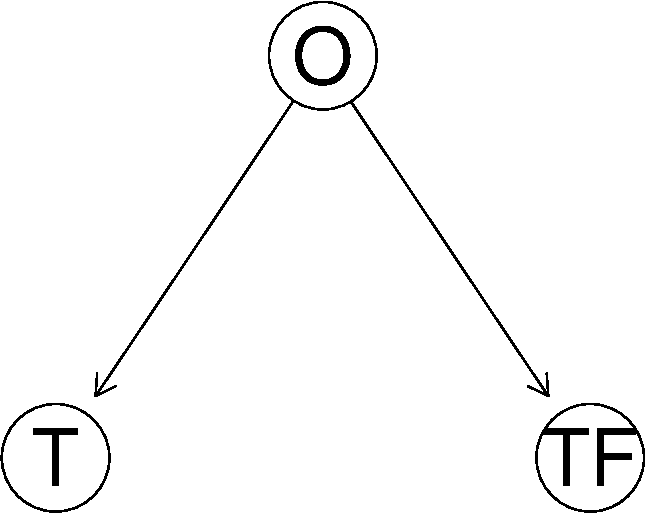
\includegraphics[width=1\linewidth]{coherencePaper32_files/figure-latex/unnamed-chunk-41-1} \end{center}
\end{subfigure} }\hfill
\begin{subfigure}[!ht]{0.6\textwidth}
\centering\begingroup\fontsize{9}{11}\selectfont
\begin{tabular}{lrr}
\toprule
\multicolumn{1}{c}{T124} & \multicolumn{2}{c}{T123} \\
  & 1 & 0\\
\midrule
\cellcolor{gray!6}{1} & \cellcolor{gray!6}{0.667} & \cellcolor{gray!6}{0.2}\\
0 & 0.333 & 0.8\\
\bottomrule
\end{tabular}
\endgroup{}
\end{subfigure}
\caption{A witness perspective for the \textsf{agreement} problem, set $A$.}
\end{figure}

\begin{figure}[H]
\hspace{2cm}\scalebox{0.6}{
\begin{subfigure}[!ht]{0.3\textwidth}


\begin{center}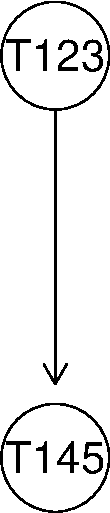
\includegraphics[width=1\linewidth]{coherencePaper32_files/figure-latex/unnamed-chunk-42-1} \end{center}
\end{subfigure}} \hfill
\begin{subfigure}[!ht]{0.6\textwidth}
\centering\begingroup\fontsize{9}{11}\selectfont

\begin{tabular}{lrr}
\toprule
\multicolumn{1}{c}{T124} & \multicolumn{2}{c}{T123} \\
  & 1 & 0\\
\midrule
\cellcolor{gray!6}{1} & \cellcolor{gray!6}{0.333} & \cellcolor{gray!6}{0.4}\\
0 & 0.667 & 0.6\\
\bottomrule
\end{tabular}
\endgroup{}
\end{subfigure}
\caption{A witness perspective for the \textsf{agreement} problem, set $B$.}
\end{figure}

\noindent Now, the resulting calculations and outcomes are in Tables \ref{tab:depthFurtherCoherence} and \ref{tab:depthFurtherDesiderata}, and the situation is no longer problematic for any of the measures.

\begin{table}[H]

\caption{\label{tab:depthFurtherCoherence}Coherence scores in a single agent version of the Depth scenario (rounded).}
\centering
\resizebox{\linewidth}{!}{
\begin{tabular}[t]{lrrrrrrrrrr}
\toprule
  & OG & OGGen & Sh & ShGen & DM & R & Fi & SZ & SLR & SL\\
\midrule
\cellcolor{gray!6}{WitnessA: T123T124 11} & \cellcolor{gray!6}{0.664} & \cellcolor{gray!6}{0.664} & \cellcolor{gray!6}{1.014} & \cellcolor{gray!6}{1.014} & \cellcolor{gray!6}{0.012} & \cellcolor{gray!6}{0.830} & \cellcolor{gray!6}{0.280} & \cellcolor{gray!6}{0.027} & \cellcolor{gray!6}{1.043} & \cellcolor{gray!6}{0.021}\\
WitnessB: T123T145 11 & 0.331 & 0.331 & 0.996 & 0.996 & -0.003 & 0.655 & -0.047 & -0.004 & 0.994 & -0.003\\
\bottomrule
\end{tabular}}
\end{table}

\begin{table}[H]

\caption{\label{tab:depthFurtherDesiderata}Desideratum satisfaction in the single agent version of the Depth scenario.}
\centering
\resizebox{\linewidth}{!}{
\begin{tabular}[t]{lllllllllll}
\toprule
  & OG & OGGen & Sh & ShGen & DM & R & Fi & SZ & SLR & SL\\
\midrule
\cellcolor{gray!6}{Depth: X$_1>$X$_2$} & \cellcolor{gray!6}{TRUE} & \cellcolor{gray!6}{TRUE} & \cellcolor{gray!6}{TRUE} & \cellcolor{gray!6}{TRUE} & \cellcolor{gray!6}{TRUE} & \cellcolor{gray!6}{TRUE} & \cellcolor{gray!6}{TRUE} & \cellcolor{gray!6}{TRUE} & \cellcolor{gray!6}{TRUE} & \cellcolor{gray!6}{TRUE}\\
\bottomrule
\end{tabular}}
\end{table}

\hypertarget{dice}{%
\subsection{Dice}\label{dice}}

\textbf{The scenario.} This scenario was offered by Schippers \& Koscholke (2019). You're either tossing a regular die, or a dodecahedron, \(X\) is the result (there is nothing particular about this choice of dice; \emph{mutatis mutandis} this should hold for other possible pairs of dice as well). Consider the coherence of:
\begin{align*} D &= \{X=2, (X=2\vee X=4)\}.\end{align*}

\noindent \textbf{Desiderata.} In this scenario posterior conditional probabilities are fixed: getting 2 or 4 logically follows from getting 2 (\(P(X=2\vee X=4|X=2)=1\)), and you always have 50\% chance to get 2 given that the outcome was 2 or 4 (\(P(X=2|X=2\vee X=4)=0.5\)). Therefore, according to Schippers \& Koscholke (2019), the coherence of the set \s{D} shouldn't change no matter which die you use.

\vspace{2mm}\begin{description}
    \item[(\s{D=const})] the coherence of \s{D} should not change.
\end{description}\vspace{2mm}

\textbf{Bayesian networks.} We'll follow the strategy similar to the one we already used. Since neither the example nor the narrations involve information about how probable it is that we're dealing with a regular die, as opposed to a dodecahedron, we avoid using a node representing this. Moreover, if at a given time the agent claims that the result is both two and (two or four), their cognitive situation at that time cannot be represented using uniform distribution for possible toss outcomes. Instead, we start with initial separate BNs for a regular die and a dodecahedron which do have uniform distributions for the \textsf{O} (outcome) node (Fig. \ref{fig:diceBN}), but when weighing the antecedent nodes which are not strictly speaking part of the narration, we use the probabilities updated in light of the narration content itself.

\begin{figure}[H]
\scalebox{1.3}{\begin{subfigure}[!ht]{0.3\textwidth}

\begin{center}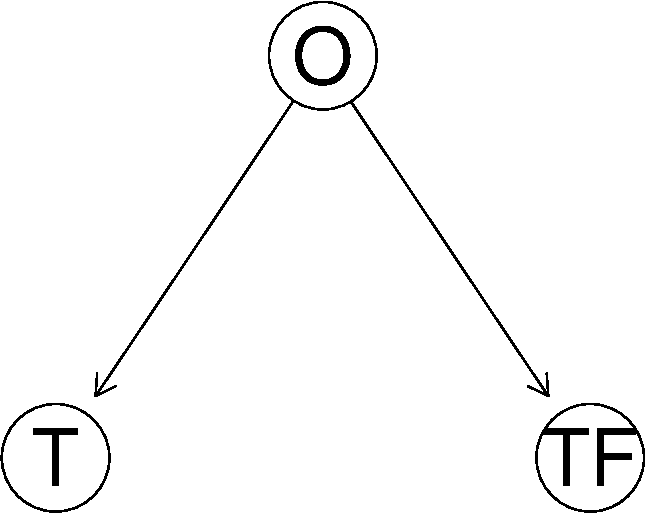
\includegraphics[width=1\linewidth]{coherencePaper32_files/figure-latex/unnamed-chunk-45-1} \end{center}
\end{subfigure}}  
\hspace{0.2cm}\begin{subfigure}[!ht]{0.25\textwidth}

\begin{tabular}{lr}
\toprule
O & Pr\\
\midrule
1 & 0.167\\
2 & 0.167\\
3 & 0.167\\
4 & 0.167\\
5 & 0.167\\
6 & 0.167\\
\bottomrule
\end{tabular}
\caption{Root CPT for the regular die.}
\end{subfigure} 
\hspace{0.2cm} \begin{subfigure}[!ht]{0.25\textwidth}

\begin{tabular}{lr}
\toprule
O & Pr\\
\midrule
1 & 0.083\\
2 & 0.083\\
3 & 0.083\\
4 & 0.083\\
5 & 0.083\\
6 & 0.083\\
7 & 0.083\\
8 & 0.083\\
9 & 0.083\\
10 & 0.083\\
11 & 0.083\\
12 & 0.083\\
\bottomrule
\end{tabular}
\caption{Root CPT for the dodecahedron.}
\end{subfigure}

\begin{subfigure}[!ht]{0.25\textwidth}

\begin{tabular}{lrrrrrr}
\toprule
\multicolumn{1}{c}{T} & \multicolumn{2}{c}{O} \\
  & 1 & 2 & 3 & 4 & 5 & 6\\
\midrule
1 & 0 & 1 & 0 & 0 & 0 & 0\\
0 & 1 & 0 & 1 & 1 & 1 & 1\\
\bottomrule
\end{tabular}


\begin{tabular}{lrrrrrr}
\toprule
\multicolumn{1}{c}{TF} & \multicolumn{2}{c}{O} \\
  & 1 & 2 & 3 & 4 & 5 & 6\\
\midrule
1 & 0 & 1 & 0 & 1 & 0 & 0\\
0 & 1 & 0 & 1 & 0 & 1 & 1\\
\bottomrule
\end{tabular}
\caption{Conditional probabilities for the regular die.}
\end{subfigure} \hfill
\scalebox{0.8}{\begin{subfigure}[!ht]{0.7\textwidth}

\begin{tabular}{lrrrrrrrrrrrr}
\toprule
\multicolumn{1}{c}{T} & \multicolumn{2}{c}{O} \\
  & 1 & 2 & 3 & 4 & 5 & 6 & 7 & 8 & 9 & 10 & 11 & 12\\
\midrule
1 & 0 & 1 & 0 & 0 & 0 & 0 & 0 & 0 & 0 & 0 & 0 & 0\\
0 & 1 & 0 & 1 & 1 & 1 & 1 & 1 & 1 & 1 & 1 & 1 & 1\\
\bottomrule
\end{tabular}


\begin{tabular}{lrrrrrrrrrrrr}
\toprule
\multicolumn{1}{c}{TF} & \multicolumn{2}{c}{O} \\
  & 1 & 2 & 3 & 4 & 5 & 6 & 7 & 8 & 9 & 10 & 11 & 12\\
\midrule
1 & 0 & 1 & 0 & 1 & 0 & 0 & 0 & 0 & 0 & 0 & 0 & 0\\
0 & 1 & 0 & 1 & 0 & 1 & 1 & 1 & 1 & 1 & 1 & 1 & 1\\
\bottomrule
\end{tabular}
\caption{\large Conditional probabilities for the dodecahedron.}
\end{subfigure}} 
\caption{BNs for the \textsf{dice} problem.}
\label{fig:diceBN}
\end{figure}

\textbf{Results.} Calculation of coherence scores of the scenarios in the respective BNs yield the result in Table \ref{tab:diceCoherence}, and the status of the desiderata is pictured in Table \ref{tab:diceDesiderata}.

\begin{table}[H]

\caption{\label{tab:diceCoherence}Coherence scores in the dice problem (rounded).}
\centering
\resizebox{\linewidth}{!}{
\begin{tabular}[t]{lrrrrrrrrrr}
\toprule
  & OG & OGGen & Sh & ShGen & DM & R & Fi & SZnarr & SLRnarr & SLnarr\\
\midrule
\cellcolor{gray!6}{Regular: TTF 11} & \cellcolor{gray!6}{0.5} & \cellcolor{gray!6}{0.5} & \cellcolor{gray!6}{3} & \cellcolor{gray!6}{3} & \cellcolor{gray!6}{0.500} & \cellcolor{gray!6}{0.75} & \cellcolor{gray!6}{0.833} & \cellcolor{gray!6}{1} & \cellcolor{gray!6}{NA} & \cellcolor{gray!6}{1}\\
Dodecahedron: TTF 11 & 0.5 & 0.5 & 6 & 6 & 0.625 & 0.75 & 0.917 & 1 & NA & 1\\
\bottomrule
\end{tabular}}
\end{table}

\begin{table}[H]

\caption{\label{tab:diceDesiderata2}Desideratum satisfaction in the dice problem.}
\centering
\resizebox{\linewidth}{!}{
\begin{tabular}[t]{lllllllllll}
\toprule
  & OG & OGGen & Sh & ShGen & DM & R & Fi & SZnarr & SLRnarr & SLnarr\\
\midrule
\cellcolor{gray!6}{Dodecahedron:  Regular $=$  Dodecahedron} & \cellcolor{gray!6}{TRUE} & \cellcolor{gray!6}{TRUE} & \cellcolor{gray!6}{FALSE} & \cellcolor{gray!6}{FALSE} & \cellcolor{gray!6}{FALSE} & \cellcolor{gray!6}{TRUE} & \cellcolor{gray!6}{FALSE} & \cellcolor{gray!6}{TRUE} & \cellcolor{gray!6}{NA} & \cellcolor{gray!6}{TRUE}\\
\bottomrule
\end{tabular}}
\end{table}

\hypertarget{discussion}{%
\section{\texorpdfstring{Discussion \label{sec:discussion}}{Discussion }}\label{discussion}}

Ultimately, all the calculations are displayed in Table \ref{tab:jointCoherences} and the desiderata yield Table \ref{tab:allResults}, with corresponding success rates (Table \ref{tab:success}).

\begin{table}[H]

\caption{\label{tab:jointCoherences}Coherence scores for all the examples.}
\centering
\resizebox{\linewidth}{!}{
\begin{tabular}[t]{lrrrrrrrr}
\toprule
  & OG & OGen & Sh & ShGen & Fit & DM & R & S\\
\midrule
\cellcolor{gray!6}{Penguins: BGP 111} & \cellcolor{gray!6}{0.010} & \cellcolor{gray!6}{0.015} & \cellcolor{gray!6}{4.000} & \cellcolor{gray!6}{2.010} & \cellcolor{gray!6}{0.453} & \cellcolor{gray!6}{0.255} & \cellcolor{gray!6}{0.255} & \cellcolor{gray!6}{0.010}\\
Penguins: BG 11 & 0.010 & 0.010 & 0.040 & 0.040 & -0.960 & -0.480 & -0.480 & -0.960\\
\cellcolor{gray!6}{Penguins: BP 11} & \cellcolor{gray!6}{0.020} & \cellcolor{gray!6}{0.020} & \cellcolor{gray!6}{2.000} & \cellcolor{gray!6}{2.000} & \cellcolor{gray!6}{0.669} & \cellcolor{gray!6}{0.255} & \cellcolor{gray!6}{0.255} & \cellcolor{gray!6}{0.010}\\
Dunnit: MGWI 1111 & 0.000 & 0.087 & 4.294 & 11.012 & 0.169 & 0.167 & 0.167 & -0.932\\
\cellcolor{gray!6}{Dunnit: MTGWI 11111} & \cellcolor{gray!6}{0.000} & \cellcolor{gray!6}{0.042} & \cellcolor{gray!6}{73.836} & \cellcolor{gray!6}{13.669} & \cellcolor{gray!6}{0.385} & \cellcolor{gray!6}{0.150} & \cellcolor{gray!6}{0.150} & \cellcolor{gray!6}{-0.100}\\
Japanese Swords 1: JO 11 & 0.004 & 0.004 & 80.251 & 80.251 & 0.976 & 0.008 & 0.008 & 0.008\\
\cellcolor{gray!6}{Japanese Swords 2: JO 11} & \cellcolor{gray!6}{0.818} & \cellcolor{gray!6}{0.818} & \cellcolor{gray!6}{9.000} & \cellcolor{gray!6}{9.000} & \cellcolor{gray!6}{0.976} & \cellcolor{gray!6}{0.800} & \cellcolor{gray!6}{0.800} & \cellcolor{gray!6}{0.889}\\
Japanese Swords 3: JO 11 & 0.818 & 0.818 & 1.080 & 1.080 & 0.286 & 0.067 & 0.067 & 0.400\\
\cellcolor{gray!6}{Robbers: MIsPMIsR 11} & \cellcolor{gray!6}{0.600} & \cellcolor{gray!6}{0.600} & \cellcolor{gray!6}{0.937} & \cellcolor{gray!6}{0.937} & \cellcolor{gray!6}{-0.143} & \cellcolor{gray!6}{-0.050} & \cellcolor{gray!6}{-0.050} & \cellcolor{gray!6}{0.600}\\
Robbers: MIsPMIsR 10 & 0.250 & 0.250 & 1.250 & 1.250 & 0.571 & 0.125 & 0.125 & -0.600\\
\cellcolor{gray!6}{Robbers: MIsPMIsR 01} & \cellcolor{gray!6}{0.250} & \cellcolor{gray!6}{0.250} & \cellcolor{gray!6}{1.250} & \cellcolor{gray!6}{1.250} & \cellcolor{gray!6}{0.571} & \cellcolor{gray!6}{0.125} & \cellcolor{gray!6}{0.125} & \cellcolor{gray!6}{-0.600}\\
Beatles: JPGRD 11111 & 0.000 & 0.202 & 0.000 & 1.423 & -0.036 & 0.025 & 0.025 & -1.000\\
\cellcolor{gray!6}{Books: AR 11} & \cellcolor{gray!6}{0.014} & \cellcolor{gray!6}{0.014} & \cellcolor{gray!6}{1.493} & \cellcolor{gray!6}{1.493} & \cellcolor{gray!6}{0.212} & \cellcolor{gray!6}{0.027} & \cellcolor{gray!6}{0.027} & \cellcolor{gray!6}{0.055}\\
Books: AR 10 & 0.009 & 0.009 & 0.945 & 0.945 & -0.127 & -0.025 & -0.025 & -0.055\\
\cellcolor{gray!6}{Books: AR 01} & \cellcolor{gray!6}{0.100} & \cellcolor{gray!6}{0.100} & \cellcolor{gray!6}{0.995} & \cellcolor{gray!6}{0.995} & \cellcolor{gray!6}{-0.101} & \cellcolor{gray!6}{-0.003} & \cellcolor{gray!6}{-0.003} & \cellcolor{gray!6}{-0.005}\\
Books: AR 00 & 0.892 & 0.892 & 1.001 & 1.001 & 0.016 & 0.001 & 0.001 & 0.005\\
\cellcolor{gray!6}{Witness: W1W2 11} & \cellcolor{gray!6}{0.451} & \cellcolor{gray!6}{0.451} & \cellcolor{gray!6}{3.551} & \cellcolor{gray!6}{3.551} & \cellcolor{gray!6}{0.771} & \cellcolor{gray!6}{0.446} & \cellcolor{gray!6}{0.446} & \cellcolor{gray!6}{0.729}\\
Witness: W3W4 11 & 0.187 & 0.187 & 0.740 & 0.740 & -0.234 & -0.110 & -0.110 & 0.494\\
\cellcolor{gray!6}{Witness: W4W5 11} & \cellcolor{gray!6}{0.365} & \cellcolor{gray!6}{0.365} & \cellcolor{gray!6}{1.260} & \cellcolor{gray!6}{1.260} & \cellcolor{gray!6}{0.218} & \cellcolor{gray!6}{0.110} & \cellcolor{gray!6}{0.110} & \cellcolor{gray!6}{0.602}\\
DepthA: T123T124 11 & 0.664 & 0.664 & 1.014 & 1.014 & 0.280 & 0.012 & 0.012 & 0.027\\
\cellcolor{gray!6}{DepthB: T123T145 11} & \cellcolor{gray!6}{0.331} & \cellcolor{gray!6}{0.331} & \cellcolor{gray!6}{0.996} & \cellcolor{gray!6}{0.996} & \cellcolor{gray!6}{-0.047} & \cellcolor{gray!6}{-0.003} & \cellcolor{gray!6}{-0.003} & \cellcolor{gray!6}{-0.004}\\
Regular: TTF 11 & 0.500 & 0.500 & 3.000 & 3.000 & 0.833 & 0.500 & 0.500 & 1.000\\
\cellcolor{gray!6}{Dodecahedron: TTF 11} & \cellcolor{gray!6}{0.500} & \cellcolor{gray!6}{0.500} & \cellcolor{gray!6}{6.000} & \cellcolor{gray!6}{6.000} & \cellcolor{gray!6}{0.917} & \cellcolor{gray!6}{0.625} & \cellcolor{gray!6}{0.625} & \cellcolor{gray!6}{1.000}\\
\bottomrule
\end{tabular}}
\end{table}

\begin{table}[H]

\caption{\label{tab:allResults}Overall desiderata satisfaction in the examples discussed).}
\centering
\resizebox{\linewidth}{!}{
\begin{tabular}[t]{lllllllll}
\toprule
  & OG & OGen & Sh & ShGen & Fit & DM & R & S\\
\midrule
\cellcolor{gray!6}{Penguins: BG$<$BGP} & \cellcolor{gray!6}{FALSE} & \cellcolor{gray!6}{TRUE} & \cellcolor{gray!6}{TRUE} & \cellcolor{gray!6}{TRUE} & \cellcolor{gray!6}{TRUE} & \cellcolor{gray!6}{TRUE} & \cellcolor{gray!6}{TRUE} & \cellcolor{gray!6}{TRUE}\\
Penguins: BP$\approx$ BGP & TRUE & TRUE & FALSE & TRUE & FALSE & TRUE & TRUE & TRUE\\
\cellcolor{gray!6}{Dunnit: Dunnit$<$Twin} & \cellcolor{gray!6}{FALSE} & \cellcolor{gray!6}{FALSE} & \cellcolor{gray!6}{TRUE} & \cellcolor{gray!6}{TRUE} & \cellcolor{gray!6}{TRUE} & \cellcolor{gray!6}{FALSE} & \cellcolor{gray!6}{FALSE} & \cellcolor{gray!6}{TRUE}\\
Swords: JO2$>$JO1 & TRUE & TRUE & FALSE & FALSE & TRUE & TRUE & TRUE & TRUE\\
\cellcolor{gray!6}{Swords: JO2$>$JO3} & \cellcolor{gray!6}{FALSE} & \cellcolor{gray!6}{FALSE} & \cellcolor{gray!6}{TRUE} & \cellcolor{gray!6}{TRUE} & \cellcolor{gray!6}{TRUE} & \cellcolor{gray!6}{TRUE} & \cellcolor{gray!6}{TRUE} & \cellcolor{gray!6}{TRUE}\\
Robbers: PR$>$P$\neg$R & TRUE & TRUE & FALSE & FALSE & FALSE & FALSE & FALSE & TRUE\\
\cellcolor{gray!6}{Robbers: PR$>$neutral} & \cellcolor{gray!6}{NA} & \cellcolor{gray!6}{NA} & \cellcolor{gray!6}{FALSE} & \cellcolor{gray!6}{FALSE} & \cellcolor{gray!6}{FALSE} & \cellcolor{gray!6}{FALSE} & \cellcolor{gray!6}{FALSE} & \cellcolor{gray!6}{TRUE}\\
Beatles: below neutral & NA & NA & TRUE & FALSE & TRUE & FALSE & TRUE & TRUE\\
\cellcolor{gray!6}{Beatles: minimal} & \cellcolor{gray!6}{TRUE} & \cellcolor{gray!6}{FALSE} & \cellcolor{gray!6}{TRUE} & \cellcolor{gray!6}{FALSE} & \cellcolor{gray!6}{FALSE} & \cellcolor{gray!6}{FALSE} & \cellcolor{gray!6}{FALSE} & \cellcolor{gray!6}{TRUE}\\
Books: AR$>$A$\neg$R & TRUE & TRUE & TRUE & TRUE & TRUE & TRUE & TRUE & TRUE\\
\cellcolor{gray!6}{Books: AR$>\neg$AR} & \cellcolor{gray!6}{FALSE} & \cellcolor{gray!6}{FALSE} & \cellcolor{gray!6}{TRUE} & \cellcolor{gray!6}{TRUE} & \cellcolor{gray!6}{TRUE} & \cellcolor{gray!6}{TRUE} & \cellcolor{gray!6}{TRUE} & \cellcolor{gray!6}{TRUE}\\
Books: $\neg$A$\neg$R$>$A$\neg$R & TRUE & TRUE & TRUE & TRUE & TRUE & TRUE & TRUE & TRUE\\
\cellcolor{gray!6}{Books: $\neg$A$\neg$R$>\neg$AR} & \cellcolor{gray!6}{TRUE} & \cellcolor{gray!6}{TRUE} & \cellcolor{gray!6}{TRUE} & \cellcolor{gray!6}{TRUE} & \cellcolor{gray!6}{TRUE} & \cellcolor{gray!6}{TRUE} & \cellcolor{gray!6}{TRUE} & \cellcolor{gray!6}{TRUE}\\
Witness: W$_1$W$_2>$W$_3$W$_4$ & TRUE & TRUE & TRUE & TRUE & TRUE & TRUE & TRUE & TRUE\\
\cellcolor{gray!6}{Witness: W$_4$W$_5>$W$_3$W$_4$} & \cellcolor{gray!6}{TRUE} & \cellcolor{gray!6}{TRUE} & \cellcolor{gray!6}{TRUE} & \cellcolor{gray!6}{TRUE} & \cellcolor{gray!6}{TRUE} & \cellcolor{gray!6}{TRUE} & \cellcolor{gray!6}{TRUE} & \cellcolor{gray!6}{TRUE}\\
Depth: X$_1>$X$_2$ & TRUE & TRUE & TRUE & TRUE & TRUE & TRUE & TRUE & TRUE\\
\cellcolor{gray!6}{Dodecahedron:  Regular $=$  Dodecahedron} & \cellcolor{gray!6}{TRUE} & \cellcolor{gray!6}{TRUE} & \cellcolor{gray!6}{FALSE} & \cellcolor{gray!6}{FALSE} & \cellcolor{gray!6}{FALSE} & \cellcolor{gray!6}{FALSE} & \cellcolor{gray!6}{FALSE} & \cellcolor{gray!6}{TRUE}\\
\bottomrule
\end{tabular}}
\end{table}

\begin{table}[H]

\caption{\label{tab:success}Success rates in the examples discussed.}
\centering
\begin{tabular}[t]{rrrrrrrr}
\toprule
OG & OGen & Sh & ShGen & Fit & DM & R & S\\
\midrule
\cellcolor{gray!6}{0.733} & \cellcolor{gray!6}{0.733} & \cellcolor{gray!6}{0.706} & \cellcolor{gray!6}{0.647} & \cellcolor{gray!6}{0.706} & \cellcolor{gray!6}{0.647} & \cellcolor{gray!6}{0.706} & \cellcolor{gray!6}{1}\\
\bottomrule
\end{tabular}
\end{table}

\hypertarget{references}{%
\section*{References}\label{references}}
\addcontentsline{toc}{section}{References}

\hypertarget{refs}{}
\begin{CSLReferences}{1}{0}
\leavevmode\vadjust pre{\hypertarget{ref-Akiba2000Shogenjis}{}}%
Akiba, K. (2000). Shogenji's probabilistic measure of coherence is incoherent. \emph{Analysis}, \emph{60}(4), 356--359. \url{https://doi.org/10.1093/analys/60.4.356}

\leavevmode\vadjust pre{\hypertarget{ref-bovens2004bayesian}{}}%
Bovens, L., \& Hartmann, S. (2004). \emph{Bayesian epistemology}. Oxford University Press.

\leavevmode\vadjust pre{\hypertarget{ref-crupi2007BayesianMeasuresEvidential}{}}%
Crupi, V., Tentori, K., \& Gonzalez, M. (2007). On {Bayesian measures} of {evidential Support}: {theoretical} and {empirical Issues}. \emph{Philosophy of Science}, \emph{74}(2), 229--252. \url{https://doi.org/10.1086/520779}

\leavevmode\vadjust pre{\hypertarget{ref-Douven2007measuring}{}}%
Douven, I., \& Meijs, W. (2007). Measuring coherence. \emph{Synthese}, \emph{156}(3), 405--425. \url{https://doi.org/10.1007/s11229-006-9131-z}

\leavevmode\vadjust pre{\hypertarget{ref-Fenton2018Risk}{}}%
Fenton, N., \& Neil, M. (2018). \emph{Risk assessment and decision analysis with bayesian networks}. Chapman; Hall.

\leavevmode\vadjust pre{\hypertarget{ref-fitelson2003ProbabilisticTheoryCoherence}{}}%
Fitelson, B. (2003). A {Probabilistic Theory} of {Coherence}. \emph{Analysis}, \emph{63}(3), 194--199.

\leavevmode\vadjust pre{\hypertarget{ref-glass2002}{}}%
Glass, D. H. (2002). Coherence, {Explanation}, and {Bayesian Networks}. In G. Goos, J. Hartmanis, J. van Leeuwen, M. O'Neill, R. F. E. Sutcliffe, C. Ryan, \ldots{} N. J. L. Griffith (Eds.), \emph{Artificial {Intelligence} and {Cognitive Science}} (Vol. 2464, pp. 177--182). {Berlin, Heidelberg}: {Springer Berlin Heidelberg}. \url{https://doi.org/10.1007/3-540-45750-X_23}

\leavevmode\vadjust pre{\hypertarget{ref-koscholke2016evaluating}{}}%
Koscholke, J. (2016). Evaluating test cases for probabilistic measures of coherence. \emph{Erkenntnis}, \emph{81}(1), 155--181. \url{https://doi.org/10.1007/s10670-015-9734-1}

\leavevmode\vadjust pre{\hypertarget{ref-Meijs2007Alleged}{}}%
Meijs, W., \& Douven, I. (2007). On the alleged impossibility of coherence. \emph{Synthese}, \emph{157}(3), 347--360. \url{https://doi.org/10.1007/s11229-006-9060-x}

\leavevmode\vadjust pre{\hypertarget{ref-Merricks1995}{}}%
Merricks, T. (1995). Warrant entails truth. \emph{Philosophy and Phenomenological Research}, \emph{55}, 841--855.

\leavevmode\vadjust pre{\hypertarget{ref-olsson2001conducive}{}}%
Olsson, E. J. (2001). Why {Coherence Is Not Truth}-{Conducive}. \emph{Analysis}, \emph{61}(3), 236--241.

\leavevmode\vadjust pre{\hypertarget{ref-olsson2005}{}}%
Olsson, E. J. (2005). The {Impossibility} of {Coherence}. \emph{Erkenntnis}, \emph{63}(3), 387--412. \url{https://doi.org/10.1007/s10670-005-4007-z}

\leavevmode\vadjust pre{\hypertarget{ref-Roche2013Coherence}{}}%
Roche, W. (2013). Coherence and probability: A probabilistic account of coherence. In M. Araszkiewicz \& J. Savelka (Eds.), \emph{Coherence: Insights from philosophy, jurisprudence and artificial intelligence} (pp. 59--91). Dordrecht: Springer.

\leavevmode\vadjust pre{\hypertarget{ref-Schippers2014Probabilistic}{}}%
Schippers, M. (2014). \emph{Probabilistic measures of coherence: From adequacy constraints towards pluralism}. \emph{191}(16), 3821--3845. \url{https://doi.org/10.1007/s11229-014-0501-7}

\leavevmode\vadjust pre{\hypertarget{ref-Schippers2019General}{}}%
Schippers, M., \& Koscholke, J. (2019). A {General Framework} for {Probabilistic Measures} of {Coherence}. \emph{Studia Logica}. \url{https://doi.org/10.1007/s11225-019-09848-3}

\leavevmode\vadjust pre{\hypertarget{ref-Schupbach2008Alleged}{}}%
Schupbach, J. N. (2008). On the alleged impossibility of bayesian coherentism. \emph{Philosophical Studies}, \emph{141}(3), 323--331. \url{https://doi.org/10.1007/s11098-007-9176-y}

\leavevmode\vadjust pre{\hypertarget{ref-Scutari2015Bayesian-Networ}{}}%
Scutari, M., \& Denis, J.-B. (2015). \emph{Bayesian networks in \textbf{{r}}}. CRC Press.

\leavevmode\vadjust pre{\hypertarget{ref-shogenji1999conducive}{}}%
Shogenji, T. (1999). Is coherence truth-conducive? \emph{Analysis}, \emph{59}(4), 338--345.

\leavevmode\vadjust pre{\hypertarget{ref-Shogenji2001Reply}{}}%
Shogenji, T. (2001). Reply to {A}kiba on the probabilistic measure of coherence. \emph{Analysis}, \emph{61}(2), 147--150. \url{https://doi.org/10.1093/analys/61.2.147}

\leavevmode\vadjust pre{\hypertarget{ref-Shogenji2006Why}{}}%
Shogenji, T. (2006). Why does coherence appear truth-conducive? \emph{Synthese}, \emph{157}(3), 361--372. \url{https://doi.org/10.1007/s11229-006-9062-8}

\leavevmode\vadjust pre{\hypertarget{ref-Siebel2004On-Fitelsons-me}{}}%
Siebel, M. (2004). On {F}itelson's measure of coherence. \emph{Analysis}, \emph{64}, 189--190.

\leavevmode\vadjust pre{\hypertarget{ref-siebel2006against}{}}%
Siebel, M. (2006). Against probabilistic measures of coherence. In \emph{Coherence, truth and testimony} (pp. 43--68). Springer.

\end{CSLReferences}

\end{document}
